%%%%%%%%%%%%%%%%%%%%%%%%%%%%%%%%%%%%%%%%%%%%%%%%%%%
%
%  New template code for TAMU Theses and Dissertations starting Fall 2016.
%
%
%  Author: Sean Zachary Roberson
%  Version 3.17.09
%  Last Updated: 9/21/2017
%
%%%%%%%%%%%%%%%%%%%%%%%%%%%%%%%%%%%%%%%%%%%%%%%%%%%
%%%%%%%%%%%%%%%%%%%%%%%%%%%%%%%%%%%%%%%%%%%%%%%%%%%%%%%%%%%%%%%%%%%%%%
%%                           TIME TO SOLUTION ESTIMATOR CHAPTER
%%%%%%%%%%%%%%%%%%%%%%%%%%%%%%%%%%%%%%%%%%%%%%%%%%%%%%%%%%%%%%%%%%%%%
 \setcounter{MaxMatrixCols}{30}
\newcommand{\tcr}[1]{\textcolor{red}{#1}}


\chapter{TIME-TO-SOLUTION ESTIMATOR \label{cha:tts}}
With the introduction of unstructured meshes and imbalanced partitions in PDT, we need an expansion of the performance model to estimate the sweep time.
In addition, before optimization of the partitioning scheme can occur, it is necessary to have an estimation tool that gives the approximate sweep time for a given partitioning scheme.
The time-to-solution estimator serves as the objective function that gets optimized, with the partitions serving as the parameter space. This chapter will detail the time-to-solution estimator, and showcase the results of 2D and 3D verification studies.

The time-to-solution estimator is written in Python 3. Python was chosen as the language for its powerful graph library, networkx \cite{networkx}.
This library gives us a wide variety of graph mathematics and is easy to use.
Before detailing the time-to-solution estimator's methodology, a description of the applicable basic graph theory is necessary.

\section{Graph Theory Applicable to the Time-to-Solution Estimator}

Graph theory is a subset of mathematics that focuses on graphs, or structures containing a set of objects that are connected in a particular manner \cite{graphtheory}.
These objects are called vertices (or nodes), and are connected by edges.
Figure~\ref{basic_graph} shows an undirected graph of 4 nodes and 4 edges. The nodes are a mathematical abstraction that can be used to represent a variety of concepts. In this dissertation, they are used to represent the subsets described in Chapter \ref{cha:lb}.
\begin{figure}[H]
\centering
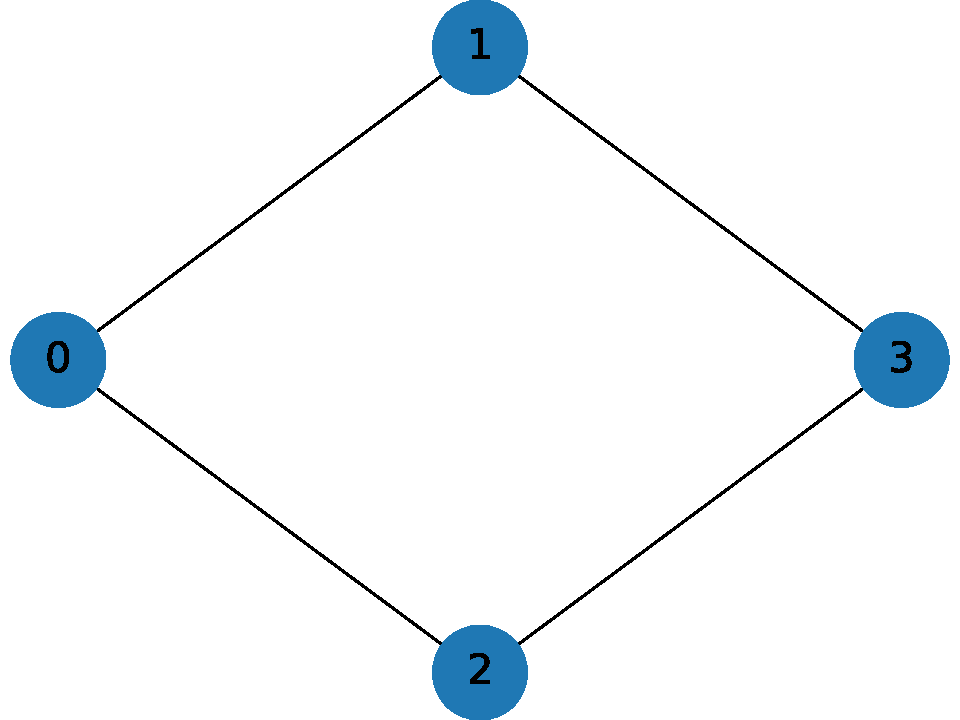
\includegraphics[scale=0.5]{../../figures/undirected_graph.pdf}
\caption{An undirected graph with 4 nodes and 4 edges. }
\label{basic_graph}
\end{figure}
Figure~\ref{basic_graph} is referred to as an undirected graph because its edges have no directional information.
If we add directional information to the edges of the graph in Fig.~\ref{basic_graph}, it becomes a directed graph, shown in Fig.~\ref{directed_graph}.
\begin{figure}[H]
\centering
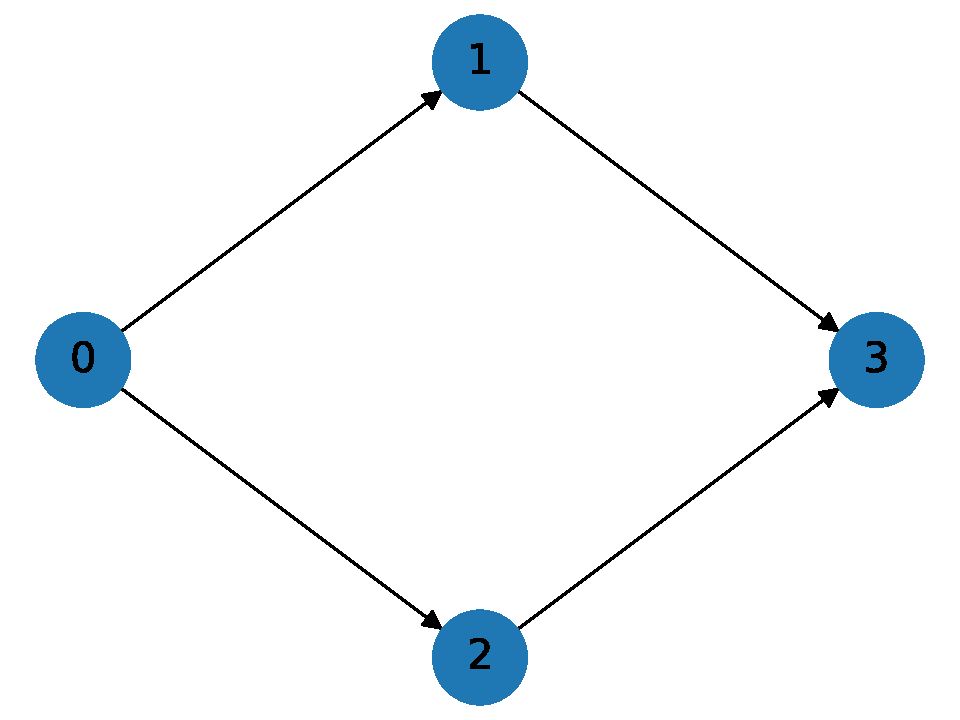
\includegraphics[scale=0.5]{../../figures/directed_graph.pdf}
\caption{A directed graph with 4 nodes and 4 edges. }
\label{directed_graph}
\end{figure}
In this dissertation, we only use Directed Acyclic Graphs (DAGs), or a graph that has no cycles.  A cycle is defined as a path on a graph that starts and ends at the same vertex. Figure~\ref{cycle_example} shows a cycle between nodes 1 and 3.
\begin{figure}[H]
\centering
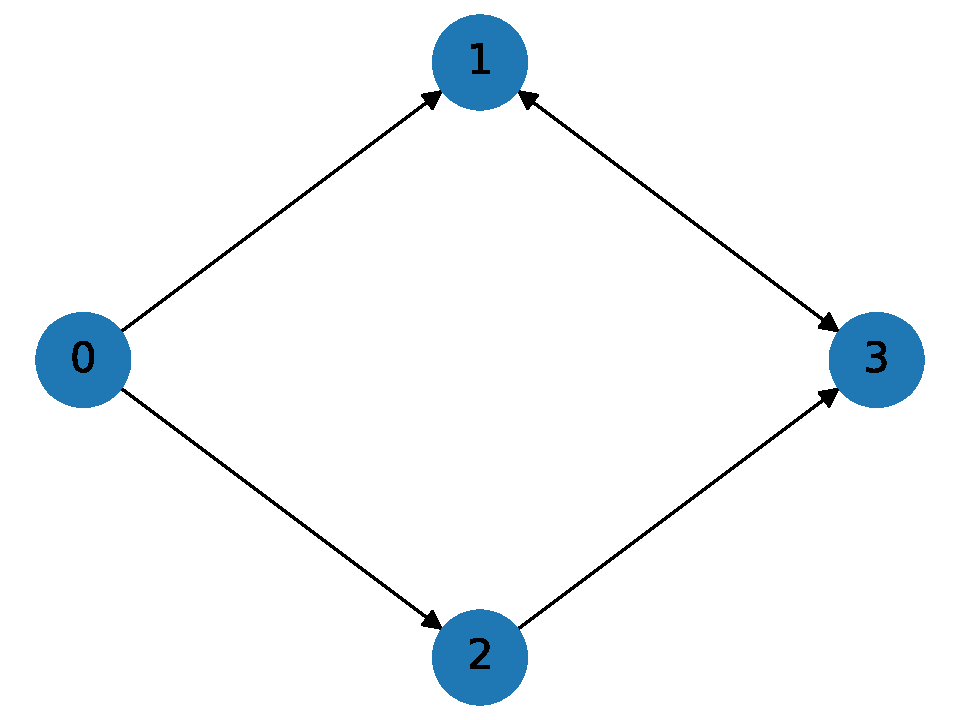
\includegraphics[scale=0.5]{../../figures/cycle_example.pdf}
\caption{A directed graph with a cycle between nodes 1 and 3.}
\label{cycle_example}
\end{figure}
We notice the edge connecting nodes 1 and 3 has a double headed arrow, representing a cycle.
Graphs with cycles can be solved for a variety of applications through the use of cycle detection and breaking algorithms, but our partitioning scheme cuts subsets in a fashion that does not allow for cyclical graphs.

Graph edges can be weighted based on the need of the application the graph is being used for. Here, we weight the graph edges to represent the time it takes to solve node A plus the communication time to node B.
Figure~\ref{weighted_directed_graph} shows a weighted directed graph.
In the context of the time-to-solution estimator, subset 1 takes 3 seconds to solve and communicate to subset 3.
\begin{figure}[H]
\centering
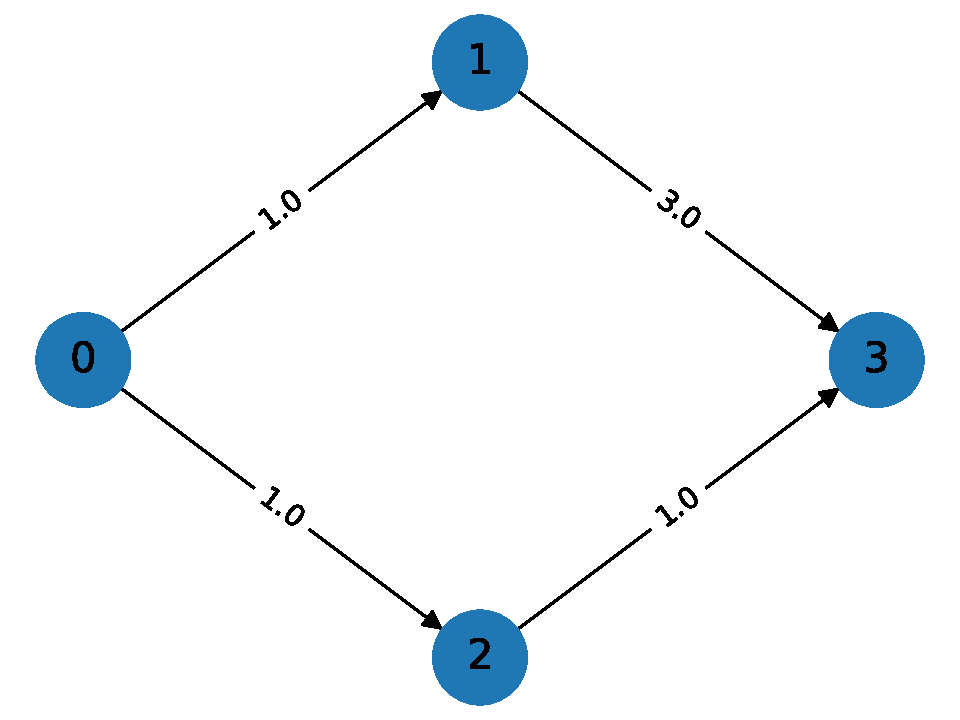
\includegraphics[scale=0.5]{../../figures/weighted_directed_graph.pdf}
\caption{A weighted directed acyclic graph with 4 nodes and 4 weighted edges.}
\label{weighted_directed_graph}
\end{figure}

The time-to-solution estimator uses Johnson's algorithm \cite{intro_to_alg,johnson_nist,johnson_johnson} to find all shortest paths between all pairs in a weighted directed graph.
The weighted shortest path is defined as the path between two nodes that has the smallest weighted sum.
For example, the shortest path between nodes 0 and 3 in Fig.~\ref{weighted_directed_graph} is $0\rightarrow 2\rightarrow 3$.

In our application, we use Johnson's algorithm to assist in calculating the longest path between two nodes in a DAG (needed in Section \ref{sec:universal}).
The longest path is found by:
\begin{enumerate}
  \item Multiplying all edge weights by -1,
  \item Using Johnson's algorithm to find the shortest (in this case the most negative) paths,
  \item Summing the original weights of this shortest path.
\end{enumerate}
Johnson's algorithm is specifically used in this process because it is capable of finding the shortest path even when edge weights are negative.

%In addition to longest path length calculation, we use an unweighted shortest path algorithm when calculating the depth-of-graph remaining (needed in Section \ref{sec:conflict}).

%\begin{figure}[H]
%\centering
%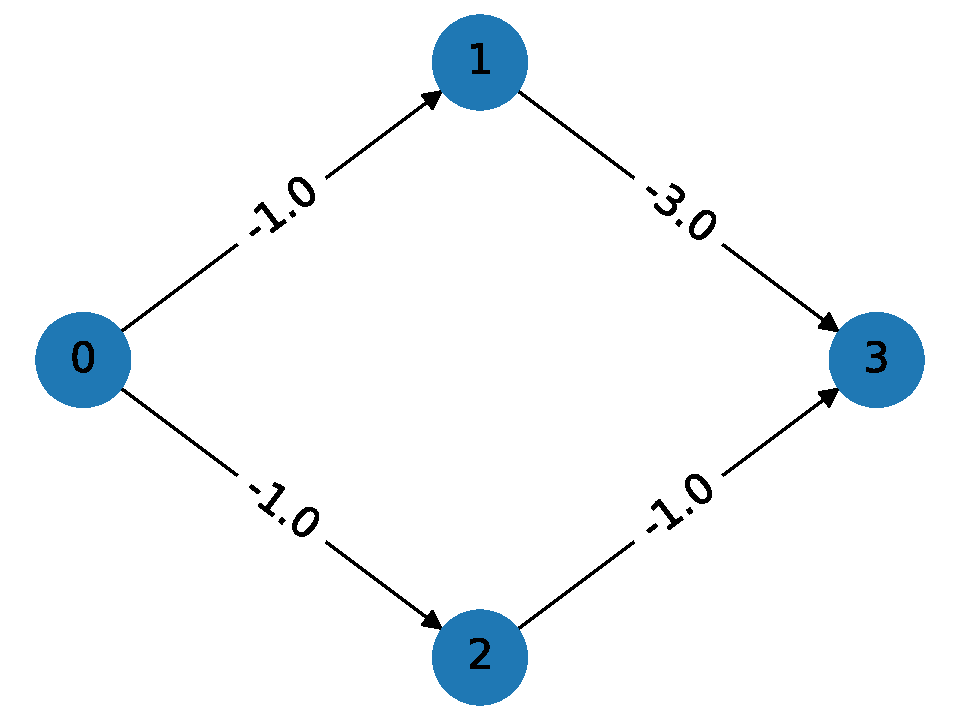
\includegraphics[scale=0.5]{../../figures/negative_weighted_directed_graph.pdf}
%\caption{The DAG in Fig.~\ref{
%\label{negative_weights}
%\end{figure}
Now that the applicable graph theory has been reviewed, we detail the methodology of the time-to-solution estimator.

%%%%%%%%%%%%%%%%%%%%%%%%%%%%%%%%%%%%%%%%%%%%%%%%%%%%%%%%%%%%%%%%%
\section{Method}
The time-to-solution estimator determines the time to sweep across a domain for a given partitioning scheme by:
\begin{enumerate}
	\item Building an adjacency matrix,
	\item Building Directed Acyclic Graphs (DAGs) from the adjacency matrix, one for each quadrant/octant,
	\item Weighting the edges of each graph based on the solve time and communication time of each subset to its neighbors,
     \item Adding and modifying graph weights based on how many anglesets are pipelined,
	\item Modifying the weights of each graph to operate on the universal timescale,
	\item Modifying the weights of each graph to reflect sweep conflicts between octants,
	\item Calculating the time to solution.
\end{enumerate}

\subsection{Building the adjacency matrices}

Before building the graph for each quadrant/octant, an adjacency matrix must be built for a given partitioning scheme. The partitioning scheme is the cut lines/planes that partition the mesh into subsets, which correspond to the processor layout.
The adjacency matrix provides connectivity information for each subset to its neighboring subset.
The adjacency building process relies on a major assumption: the z dimension has partitions all the way across the domain, then the x dimension has partitions per plane, then the y dimension has partitions per plane per column.
In future work, these three dimensions can be made interchangeable, but in the present work, this ordering is fixed.

Figure~\ref{25basematrix} shows a partitioning scheme for 3 subsets each in the x and y dimensions with its corresponding adjacency matrix.

\begin{figure}[H]
\begin{minipage}[c]{0.5\textwidth}
\centering
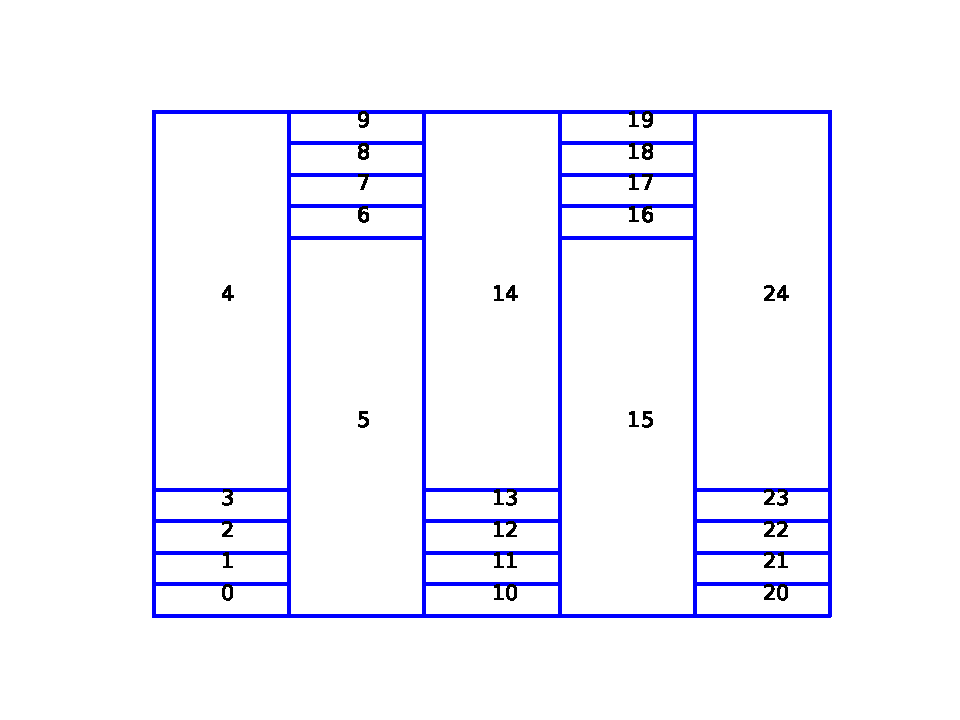
\includegraphics[scale=0.7]{../../figures/boundaries_worst.pdf}
\end{minipage}
\begin{minipage}[c]{0.6\textwidth}
\centering
\scalebox{0.75}{
$\begin{pmatrix}
0&1&0&1&0&0&0&0&0\\
1&0&1&1&0&0&0&0&0\\
0&1&0&1&1&1&0&0&0\\
1&1&1&0&1&0&1&1&1\\
0&0&1&1&0&1&0&0&1\\
0&0&1&0&1&0&0&0&1\\
0&0&0&1&0&0&0&1&0\\
0&0&0&1&0&0&1&0&1\\
0&0&0&1&1&1&0&1&0\\
\end{pmatrix}$}
\end{minipage}
\caption{A 3x3 subset partitioning scheme and its corresponding adjacency matrix.}
\label{25basematrix}
\end{figure}

\subsection{Building the directed acyclic graphs (DAGs)}

The adjacency matrices give us directed connectivity information in order to build our graphs. This process differs slightly from 2D to 3D. Both processes use on networkx's DiGraph function to build the DAGs.

\subsubsection{Building the 2D graphs}
In two dimensions, we build four graphs corresponding to four quadrants.
We define the quadrants in the following manner:
\begin{itemize}
  \item Quadrant 0: $\Omega_x > 0$, $\Omega_y > 0$
  \item Quadrant 1: $\Omega_x > 0$, $\Omega_y < 0$
  \item Quadrant 2: $\Omega_x < 0$, $\Omega_y > 0$
  \item Quadrant 3: $\Omega_x < 0$, $\Omega_y < 0$
\end{itemize}
Figure~\ref{quadrant_layout} illustrates this numbering.
\begin{figure}[H]
\centering
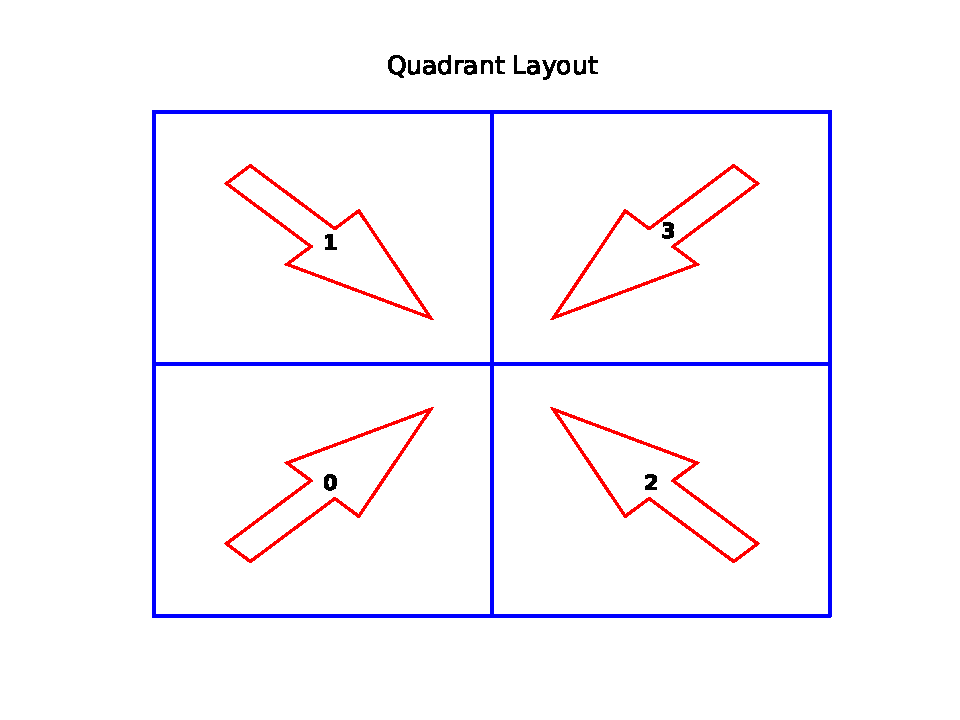
\includegraphics{figures/quadrant_layout.pdf}
\caption{The quadrant layout for 2D problems.}
\label{quadrant_layout}
\end{figure}
The initial adjacency matrix we obtain can be immediately used to build the graphs for quadrants 0 and 3 by using networkx's DiGraph function.
We feed the upper triangular portion of the adjacency matrix to DiGraph to get the quadrant 0 graph, and the lower triangular portion to get the quadrant 3 graph.
Utilizing the same partitioning scheme shown in Fig.~\ref{25basematrix}, pull the upper triangular and lower triangular portions of the matrix, shown in Fig.~\ref{25baseportionmatrices}.
\begin{figure}[H]
\begin{minipage}[c]{0.5\textwidth}
\centering
\scalebox{0.75}{
$\begin{pmatrix}
0&1&0&1&0&0&0&0&0\\
0&0&1&1&0&0&0&0&0\\
0&0&0&1&1&1&0&0&0\\
0&0&0&0&1&0&1&1&1\\
0&0&0&0&0&1&0&0&1\\
0&0&0&0&0&0&0&0&1\\
0&0&0&0&0&0&0&1&0\\
0&0&0&0&0&0&0&0&1\\
0&0&0&0&0&0&0&0&0\\
\end{pmatrix}$}
\end{minipage}
\begin{minipage}[c]{0.5\textwidth}
\centering
\scalebox{0.75}{
$\begin{pmatrix}
0&0&0&0&0&0&0&0&0\\
1&0&0&0&0&0&0&0&0\\
0&1&0&0&0&0&0&0&0\\
1&1&1&0&0&0&0&0&0\\
0&0&1&1&0&0&0&0&0\\
0&0&1&0&1&0&0&0&0\\
0&0&0&1&0&0&0&0&0\\
0&0&0&1&0&0&1&0&0\\
0&0&0&1&1&1&0&1&0\\
\end{pmatrix}$}
\end{minipage}
\caption{The upper triangular (left) and lower triangular (right) portions of the adjacency matrix in Fig.~\ref{25basematrix}.}
\label{25baseportionmatrices}
\end{figure}
Figure~\ref{25_q0q3graphs} shows the the DAGS associated with quadrants 0 and 3, built from the adjacency matrices in Fig.~\ref{25baseportionmatrices}.
\begin{figure}[H]
\begin{minipage}[c]{0.5\textwidth}
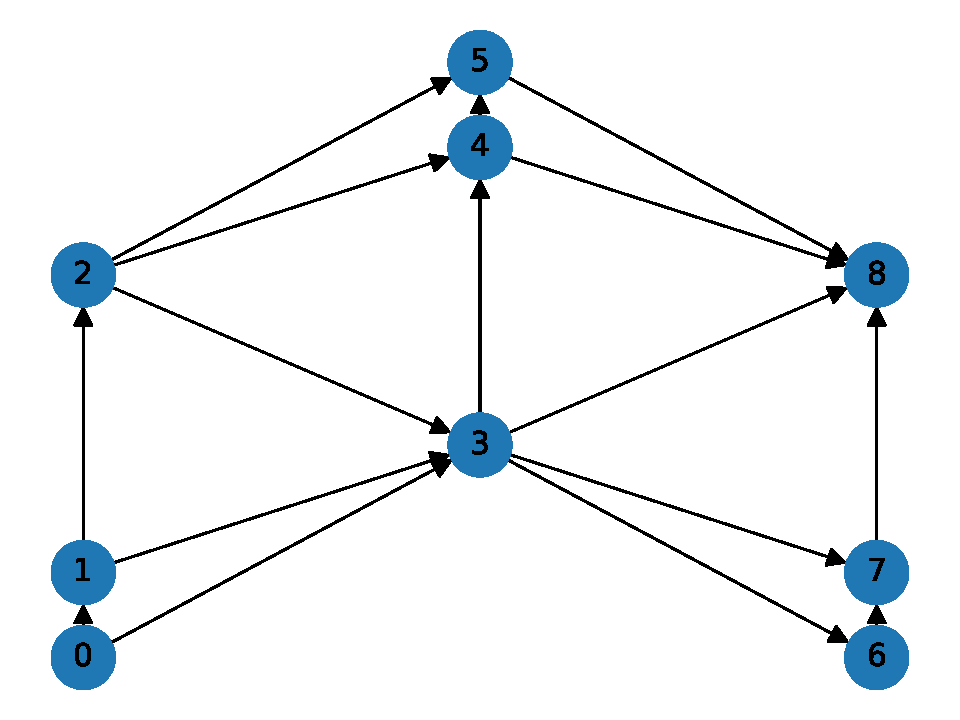
\includegraphics[scale=0.5]{../../figures/9_graph0.pdf}
\end{minipage}
\begin{minipage}[c]{0.5\textwidth}
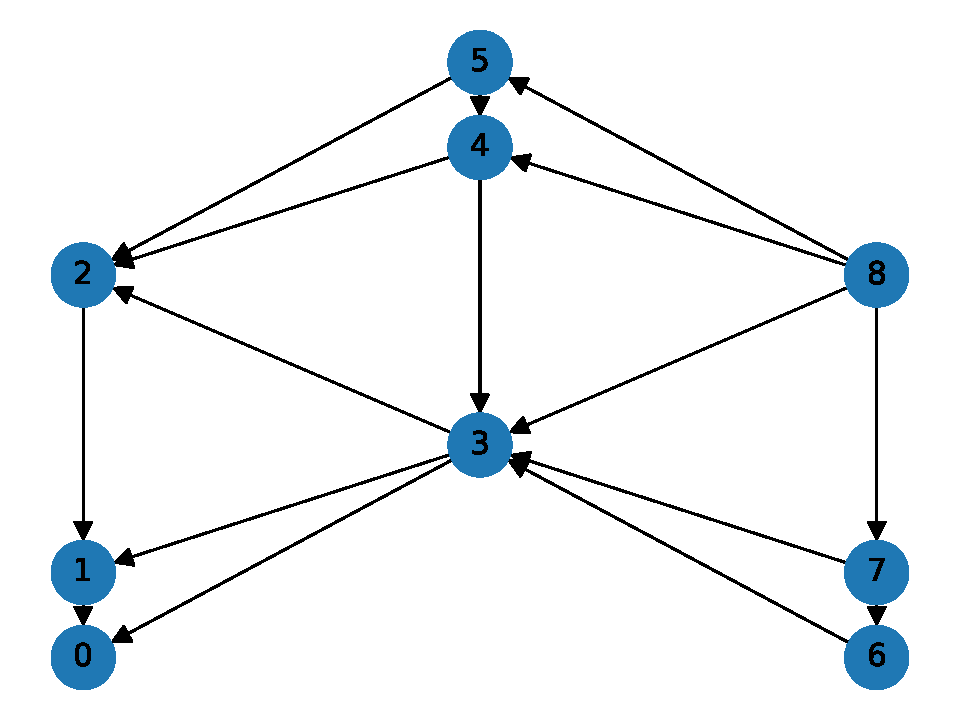
\includegraphics[scale=0.5]{../../figures/9_graph3.pdf}
\end{minipage}
\caption{The quadrant 0 DAG (left) and the quadrant 3 DAG (right).}
\label{25_q0q3graphs}
\end{figure}
Upon inspection of these two DAGs, we see that they show the expected connectivity, dependency, and opposing sweep ordering.
Quadrant 0 starts its sweep from subset 0, finishing at subset 8, and quadrant 3 starts its sweep from subset 8, finishing at subset 0.

To obtain the graphs for quadrants 1 and 2, a ``flipped'' version of the adjacency matrix is necessary.
We temporarily renumber the subsets starting from the top left corner, and increasing down each column, as shown in Fig.~\ref{25flippedmatrix}.
\begin{figure}[H]
\begin{minipage}[c]{0.5\textwidth}
\centering
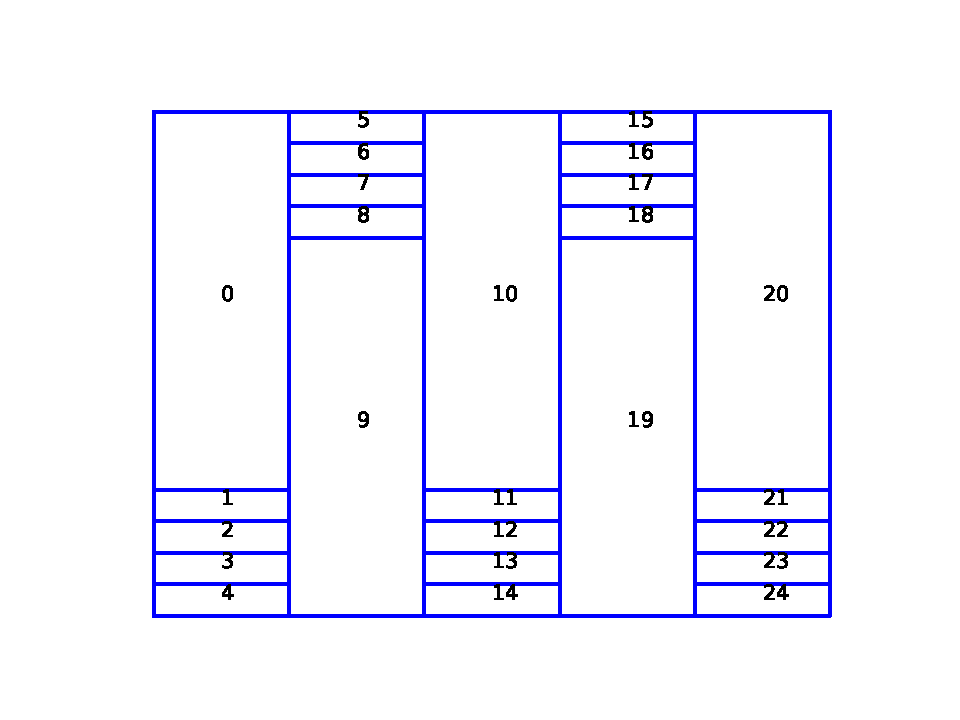
\includegraphics[scale=0.7]{../../figures/boundaries_worst_flipped.pdf}
\end{minipage}
\begin{minipage}[c]{0.5\textwidth}
\centering
\scalebox{0.75}{
$\begin{pmatrix}
0&1&0&1&1&1&0&0&0\\
1&0&1&0&0&1&0&0&0\\
0&1&0&0&0&1&0&0&0\\
1&0&0&0&1&0&1&0&0\\
1&0&0&1&0&1&1&0&0\\
1&1&1&0&1&0&1&1&1\\
0&0&0&1&1&1&0&1&0\\
0&0&0&0&0&1&1&0&1\\
0&0&0&0&0&1&0&1&0\\
\end{pmatrix}$}
\end{minipage}
\caption{The flipped subset ordering and corresponding ``flipped'' adjacency matrix for the partitioning scheme in Fig.~\ref{25basematrix}.}
\label{25flippedmatrix}
\end{figure}
We then get the upper triangular and lower triangular portions of the flipped adjacency matrix to get the connectivity and dependency information for quadrants 1 and 2.
We feed the triangular matrices into networkx's DiGraph function, along with a mapping of the flipped subset ids to the original subset ids (shown in Fig.~\ref{25basematrix}). Figure~\ref{25_q1q2graphs} shows the DAGs for quadrants 1 and 2.
\begin{figure}[H]
\begin{minipage}[c]{0.5\textwidth}
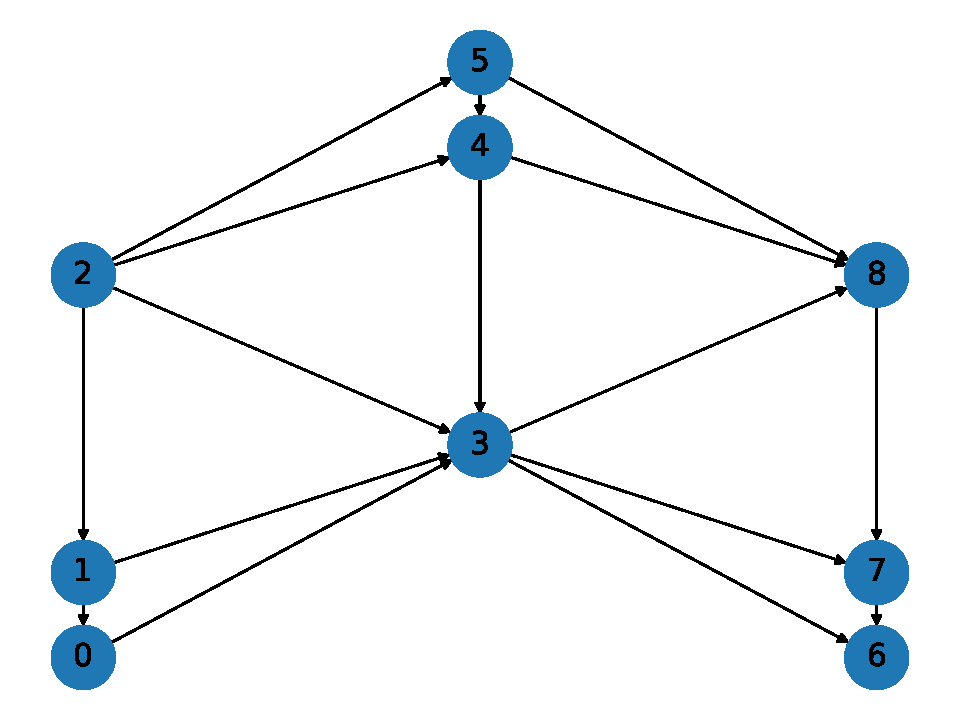
\includegraphics[scale=0.5]{../../figures/9_graph1.pdf}
\end{minipage}
\begin{minipage}[c]{0.5\textwidth}
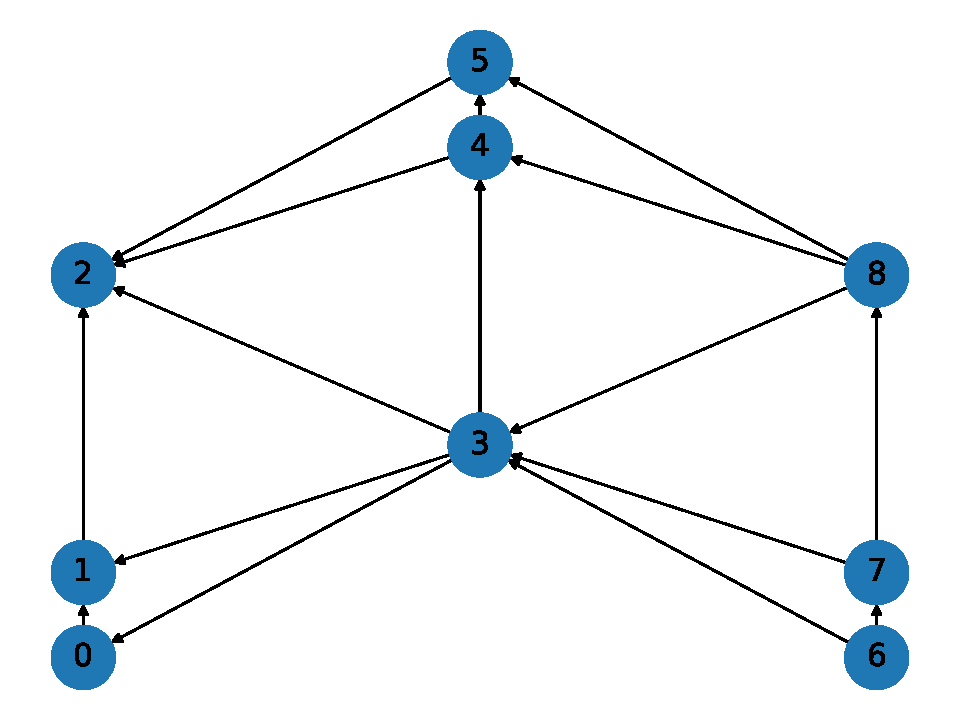
\includegraphics[scale=0.5]{../../figures/9_graph2.pdf}
\end{minipage}
\caption{The quadrant 1 DAG (left) and the quadrant 2 DAG(right).}
\label{25_q1q2graphs}
\end{figure}
Upon inspection of these two DAGs, we see that they show the expected connectivity, dependency, and opposing sweep ordering.
Quadrant 1 starts its sweep from subset 2, finishing at subset 6, and quadrant 2 starts its sweep from subset 6, finishing at subset 2.

%Weighting the TDGS
\subsection{Weighting the task dependence graphs}

Each graph is weighted to reflect the solve time and communication time of each node to its neighbors. Explicitly, the edge weight between node A and node B represents the solve time of node A added to the time it takes to communicate boundary information from nod A to node B. Equation \ref{weight_function} shows how the weights are calculated:
\begin{equation}
\text{weight} = \text{mcff}\cdot [T_{wu} + N_n\cdot \text{latency}\cdot M_L + T_{\text{comm}}\cdot N_b\cdot A_m\cdot upbc + \cdot N_c\cdot (T_c + A_m\cdot (T_m + T_g))],
\label{weight_function}
\end{equation}
where:
\begin{itemize}
  \item mcff = the Multi-Core Fudge Factor, a corrective factor that accounts for performance drop-off from 1 to 8 cores,
  \item $T_{wu}$ = the time to get into the sweep operator,
  \item $N_n$ = the number of neighbors this node has to communicate to,
  \item latency = the machine specific communication latency,
  \item $M_L$ = the machine specific latency multiplier,
  \item $T_{\text{comm}}$ = the communication time per double,
  \item $N_b$ = the number of boundary cells shared by node A and node B,
  \item $A_m$ = the number of angles node A has to solve prior to communicating,
  \item $upbc$ = the number of boundary unknowns per boundary cell,
  \item $N_c$ = the number of cells in node A,
  \item $T_c$ = the time spent solving cell-specific work,
  \item $T_m$ = the time spent solving angle-specific work,
  \item $T_g$ = the time spent solving group-specific work.
\end{itemize}
The weighting function is based on PDT's performance model \cite{mpadams2013,mpadams2015,mpadamsjcp}, which is specific to how PDT solves the transport sweep. The cost function can be modified based on different sweep methodologies if a user desires.

As shown in Eq. \ref{weight_function}, a crucial part of determining the weight of each edge is knowing the number of cells each subset has, and the amount of shared boundary cells with each neighbor. Given a mesh density, the number of cells per subset is given by Eq \ref{cellspersubset}:
\begin{equation}
   \text{cells per subset} = \int_{x_i}^{x_{i+1}} \int_{y_j}^{y_{j+1}} \int_{z_k}^{z_{k+1}} \text{mesh density } dx dy dz,
\label{cellspersubset}
\end{equation}
where the integral bounds represent the cut plane coordinates that form the subset.
Equations \ref{nxy}-\ref{nyz} calculate the boundary cells along each face in 3D:
\begin{align}
n_{xy} &= \Big(\frac{N_c}{V}\Big)^{2/3}\cdot L_x\cdot L_y \label{nxy}, \\
n_{xz} &= \Big(\frac{N_c}{V}\Big)^{2/3}\cdot L_x\cdot L_z \label{nxz}, \\
n_{yz} &= \Big(\frac{N_c}{V}\Big)^{2/3}\cdot L_y\cdot L_z \label{nyz},
\end{align}
where $N_c$ is the number of cells in the subset, $V$ is the subset volume, and $L_d$ is the length of the subset in dimension $d$.
Equations \ref{nx} and \ref{ny} show the 2-dimensional equivalents to \ref{nxy}-\ref{nyz}:
\begin{align}
n_x &= \Big(\frac{N_c}{A}\Big)^{1/2}\cdot L_x, \label{nx} \\
n_y &= \Big(\frac{N_c}{A}\Big)^{1/2}\cdot L_y, \label{ny}
\end{align}
where $A$ is the subset area. Equations \ref{cellspersubset}-\ref{ny} are exact for structured meshes.
However, unstructured meshes do not necessarily have an easily integrable mesh density function to calculate the cells per subset.

\subsubsection{Determining the cells per subset for unstructured meshes}
To get the cells per subset for unstructured meshes we require the vertex data of the mesh, as well as which vertices form each cell in the mesh.
With this data, we take advantage of Python's shapely library \cite{shapely} to determine which cells lie in each subset. From the vertex and cell data of the mesh, we build a lightweight version of each cell as a shapely Polygon.\\
\noindent
For each subset we:
\begin{enumerate}
  \item Loop over the Polygons.
  \item For each polygon, check if the Polygon is within the subset. If it is, add it to the cells in that subset.
  \item If it is not within the subset, check if the Polygon intersects the subset.
  \item If it does intersect the subset, check if it lies on a natural boundary and is outside the subset.
  \item If it is not on a natural boundary and truly intersects the subset, then this Polygon's intersection with the subset forms a new cell,  and is added to the total number of cells in that subset.
\end{enumerate}
%%%%%%%%%%Table
Table \ref{2x2_cellcount} tabulates the cells count per subset for the time-to-solution estimator and PDT for the mesh in Fig.~\ref{partitioning_example} partitioned into 2 subsets in each dimension with regular cuts.
\begin{table}[H]
\centering
\caption{The cell count per subset for the time-to-solution estimator and PDT for the mesh in Fig.~\ref{partitioning_example} partitioned into 2 subsets in each dimension with regular cuts.}
\label{2x2_cellcount}
\begin{tabular}{c|c|c}
\textbf{Subset} & \textbf{Cell Count TTS} & \textbf{Cell Count PDT} \\ \hline
0 & 185 & 185 \\ \hline
1 & 25 & 25 \\ \hline
2 & 25 & 25 \\ \hline
3 & 185 & 185
\end{tabular}
\end{table}

Figure~\ref{ubp_7x7} shows the mesh in Fig.~\ref{partitioning_example} partitioned into 7 subsets in each dimension with load-balanced-by-dimension cuts. This mesh has many subsets that slice through cells, creating new cells. Figure~\ref{cell_comp} shows the cell counts per subset from PDT and the time-to-solution estimator are in perfect agreement.
%%%%%%%%%%%%%%%%%
\begin{figure}[H]
\centering
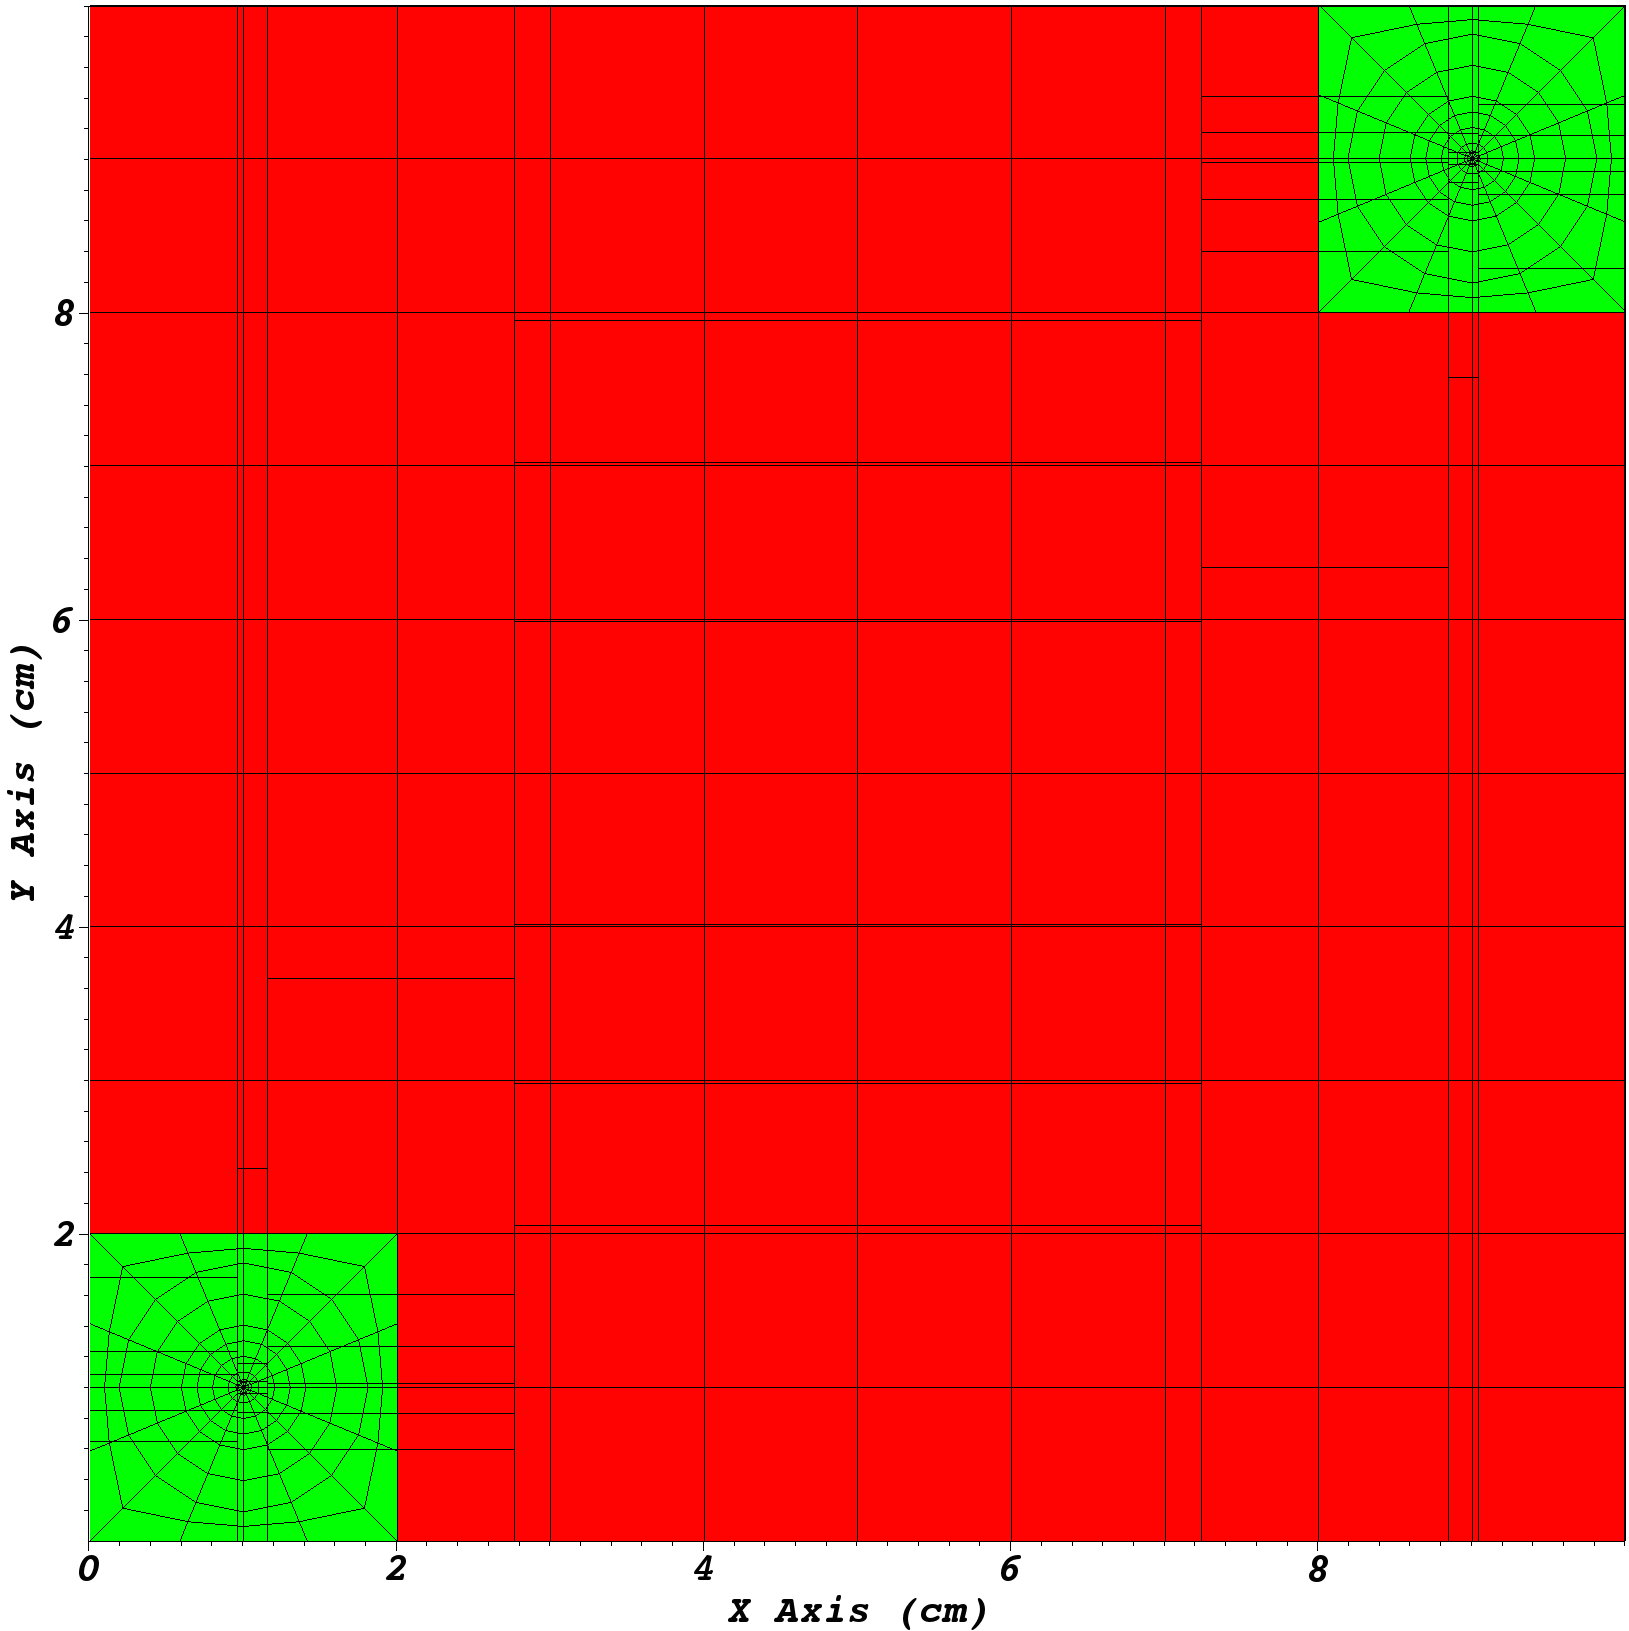
\includegraphics[scale=0.15]{../figures/spiderweb_7x7_lbd.png}
\caption{The mesh in Fig.~\ref{partitioning_example} partitioned into 7 subsets in each dimension with load-balanced-by-dimension cuts. $f = 1.49$}
\label{ubp_7x7}
\end{figure}
\begin{figure}[H]
\centering
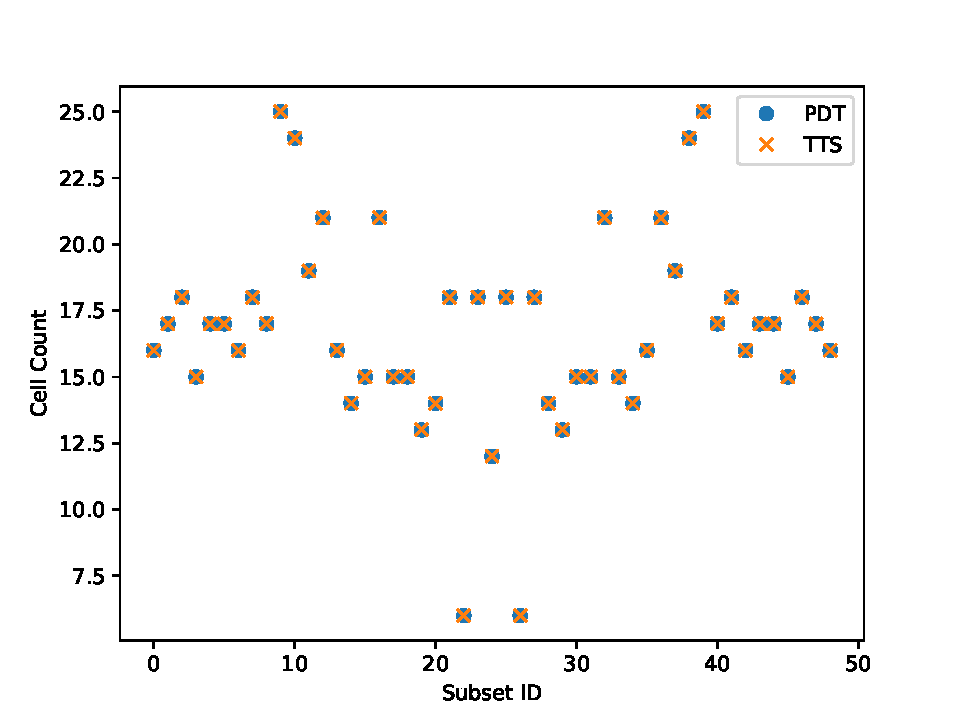
\includegraphics[scale=0.75]{../figures/spiderweb_cell_comp_7x7.pdf}
\caption{The cell count per subset for the mesh in Fig.~\ref{ubp_7x7} from PDT and the time-to-solution estimator.}
\label{cell_comp}
\end{figure}

With confidence in the cell count per subset in the time-to-solution estimator matching PDT, we make an assumption that the cells in each subset are close to uniformly distributed. This allows us to continue to use Eqs. \ref{nxy}-\ref{ny} to calculate the boundary cells in each subset.

With this information, we compute all weights in each graph according to Eq. \ref{weight_function}.
Once graphs are weighted, we add and modify edge weights for the number of angles pipelined per octant/quadrant.

\subsection{Adding graphs for angular pipelining}

If there are angles to be pipelined, the time-to-solution estimator adds a new set of graphs for each additional angle to be pipelined. For example, if there are two anglesets per octant, this would results in 16 graphs, or 1 graph per octant per angleset. Figure~\ref{angular_pipeline} shows the graphs for two anglesets for a quadrant. A ``dummy'' node with a value of -2 is added in order to have an incoming edge for the first subset's node. The value of this incoming edge represents when that angleset starts its sweep.
\begin{figure}[H]
\begin{minipage}[c]{0.5\textwidth}
\centering
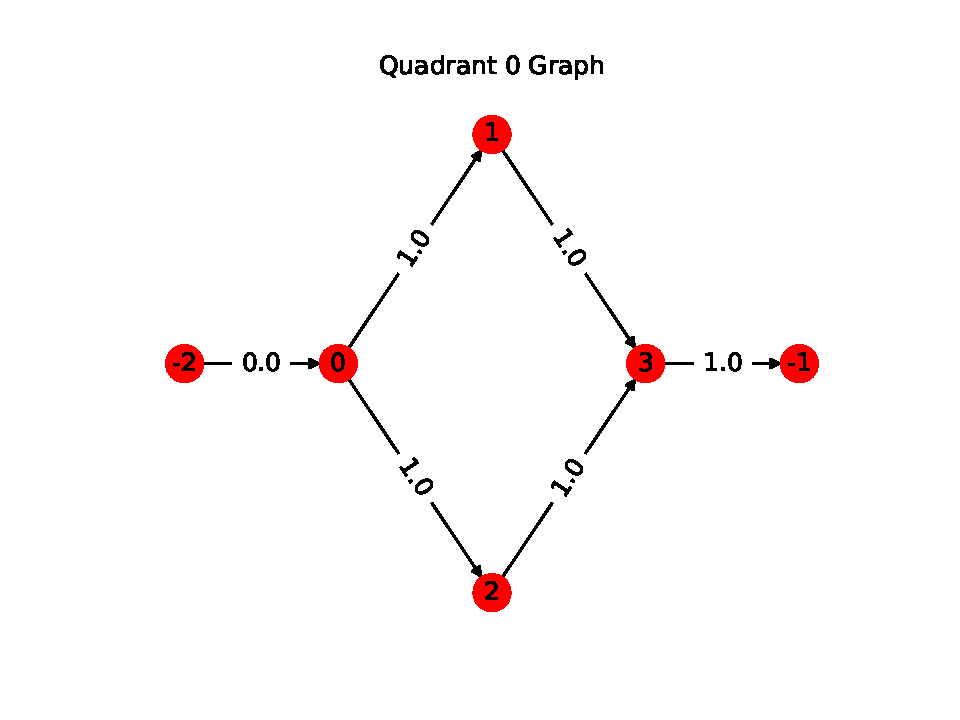
\includegraphics[scale=0.6]{../../figures/q0_postpipeline.pdf}
\end{minipage}
\begin{minipage}[c]{0.5\textwidth}
\centering
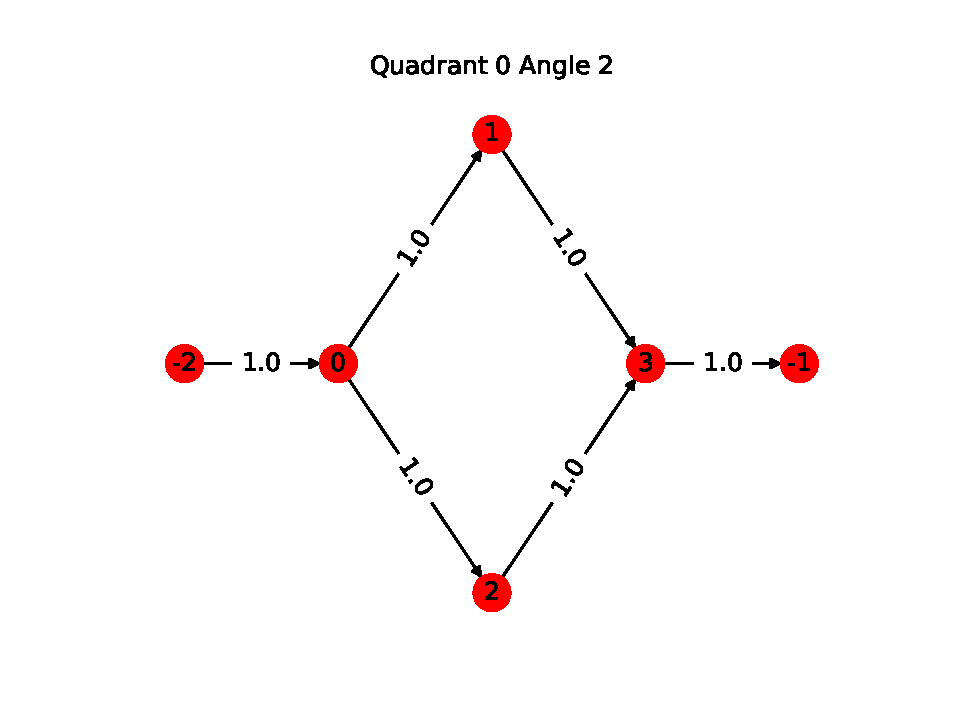
\includegraphics[scale=0.6]{../../figures/q4_postpipeline.pdf}
\end{minipage}
\caption{The graphs for the first (left) and second (right) anglesets}
\label{angular_pipeline}
\end{figure}

\subsection{Modifying the weights of each graph to reflect a universal timescale}\label{sec:universal}

Once we have our full set of graphs with angular pipelining accounted for, we set up each graph to reflect a universal timescale, with the goal of knowing when each node in each graph is ready to solve.
For each node in each graph, we:
\begin{enumerate}
  \item Calculate the longest path to the node,
  \item Sum the weights of the edges along the longest path,
  \item Set all incoming edge values to the node to the sum of the longest path.
\end{enumerate}
The incoming edges to each node in each graph now reflect the time at which a node is ready to solve. This universal edge weighting is used for detecting and resolving conflicts during the sweep. It is important to note that our DAGs are now task dependence graphs (TDGs). We now know which node is ready to solve at each time $t$, which provides us with a schedule. Figure~\ref{universal} shows a simple example of a DAG becoming a TDG.
\begin{figure}[H]
  \begin{minipage}[c]{0.5\textwidth}
    \centering
    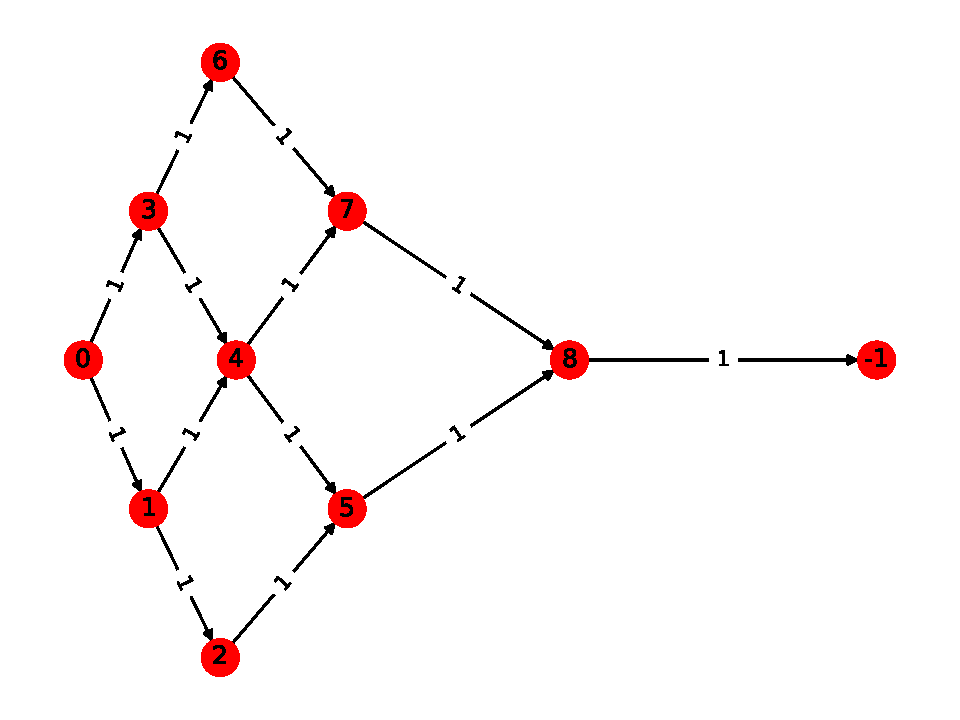
\includegraphics[scale=0.5]{../../figures/G_pre_universal.pdf}
  \end{minipage}
  \begin{minipage}[c]{0.5\textwidth}
    \centering
    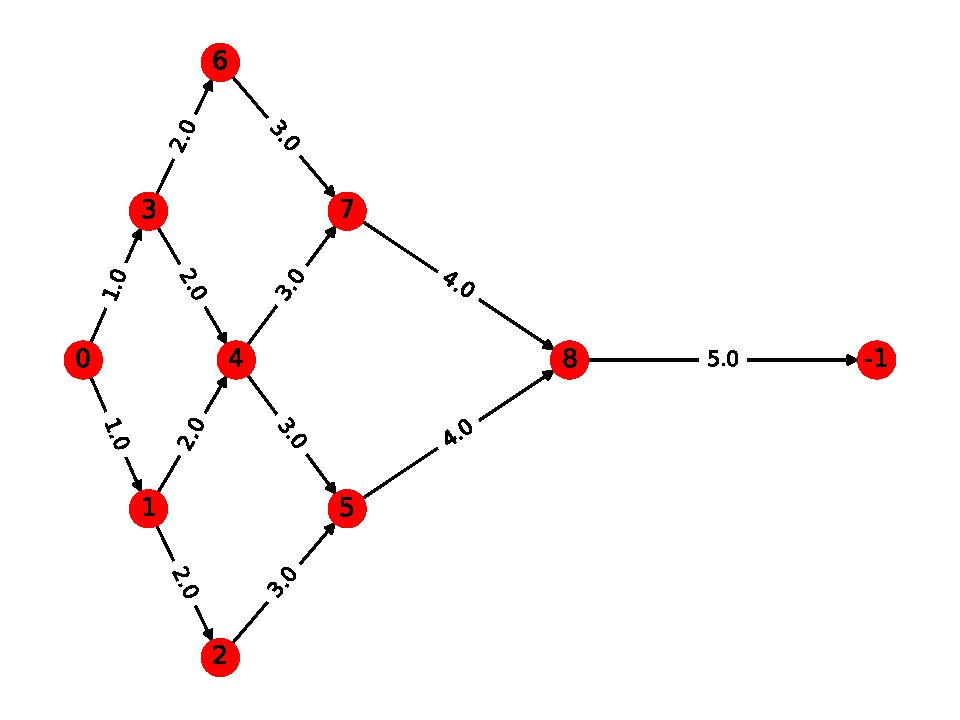
\includegraphics[scale=0.5]{../../figures/G_universal.pdf}
  \end{minipage}
  \caption{A TDG before (left) and after (right) universal edge weighting is applied.}
   \label{universal}
\end{figure}

\subsection{Modifying the weights of each graph to reflect conflict resolution}\label{sec:conflict}

At this point in the time-to-solution estimation process, we have a graph per octant/quadrant per angleset, with each graph weighted on a universal time scale.
For each node in every graph, the incoming edges to the node represent the time $t$ that it is ready to solve at.
The time to solution is best summarized as a ``marching'' process:
    \begin{enumerate}
      \item Set $t = 0$.
      \item At time $t$, find the nodes that are ready to solve or have been solving across all graphs.
      \item If at time $t$, multiple graphs are solving the same node, they are in conflict.
      \item The graph that ``wins'' the conflict does not have its weights modified, while the graph(s) that lose the conflict modify their downstream weights according to how long they are delayed.
      \item Update $t$ to the time value of the next node that's ready to solve in any graph.
      \item Repeat steps 2-5 until all graphs are finished sweeping.
    \end{enumerate}

When a conflict is detected, the time-to-solution estimator uses a first-come-first-serve conflict resolution method.
The first graph to arrive to a node will begin solving it, and the remaining graphs that arrive while it is being solved will incur a delay.
The delay is reflected in the remaining graphs by adding the delay as a weight to the applicable edge and all downstream edges in the losing graphs.

If two or more graphs arrive to a node at the same time, the octant with the greater remaining depth-of-graph (simply, more work remaining), wins.
In the case of a tie in the depth-of-graph remaining, the graph with the priority direction wins according to the following rules:
\begin{enumerate}
    \item The graph with $\Omega_x > 0$ wins,
	\item If multiple graphs have $\Omega_x > 0$, then the task with $\Omega_y > 0$ wins,
	\item If multiple graphs have $\Omega_y > 0$, then the task with $\Omega_z > 0$ wins.
\end{enumerate}
The delay is once again added to the applicable edge's weight and all downstream edges' weights.

\subsection{Estimating the final time-to-solution}

Once all graphs have had their weights modified for conflicts, the graphs now reflect a schedule. The incoming edges to each node in each graph represent what time they are ready to solve. The final weight (the outgoing edge of the final subset) in each graph represents the time it takes for that graph to sweep across its domain. The maximum final weight across all graphs represents the estimate for the time-to-solution for the problem.

\section{2D Verification}

A theoretical study in 2D is run to verify the time-to-solution estimator for 2D partitioning schemes with perfectly balanced partitions. The test problems are verified against a code written by Jean Ragusa that uses a depth-of-graph with an octant priority tie breaker scheduler in two dimensions. The verification study consists of the following problems:
\begin{enumerate}
	\item 2x2 to 10x10 subsets in x and y with regular partitions and 1 to 6 anglesets per quadrant.
	\item 2x2 to 10x10 subsets in x and y with ``mildly random'' partitions and 1 to 6 anglesets per quadrant.
	\item  2x2 to 10x10 subsets in x and y with ``random'' partitions and 1 to 6 anglesets per quadrant.
	\item  2x2 to 10x10 subsets in x and y with probable worst-case partitions and 1 to 6 anglesets per quadrant.
\end{enumerate}

``Mildly random'' partitions keep the cut lines uniformly distributed in x, while the y cut lines vary slightly around the uniformly distributed cut lines of the regular partitions. Figure~\ref{mild_random_partitions} shows examples of this partitioning style. ``Random'' partitions possesses no such limitations on either set of cut lines, as shown by Fig.~\ref{random_partitions}. The ``mildly random'' and ``random'' partition styles mimic likely partitioning schemes we can expect from load-balancing-by-dimension.

Figures \ref{regular_partitions}, \ref{mild_random_partitions}, \ref{random_partitions}, \ref{worst_partitions} show the four partitioning schemes and Figs. \ref{regular_verification}, \ref{mild_random_verification}, \ref{random_verification}, \ref{worst_verification} show the results of the verification study for each partitioning scheme. In the results, a stage is defined as the time it takes to solve all cells in a subset for an angle, and communicate the boundary information to neighboring subsets.

\subsection{Regular Partitions}

Figure~\ref{regular_partitions} shows four examples of the regular partitioning scheme used for the first part of the verification study. Cut lines in both dimensions go all the way across the domain. This reflects the partitioning scheme after the original load balancing algorithm described in Section \ref{sec:og_lb} is used.

%Regular partitions
\begin{figure}[H]
\centering
\begin{subfigure}[b]{0.45\textwidth}
  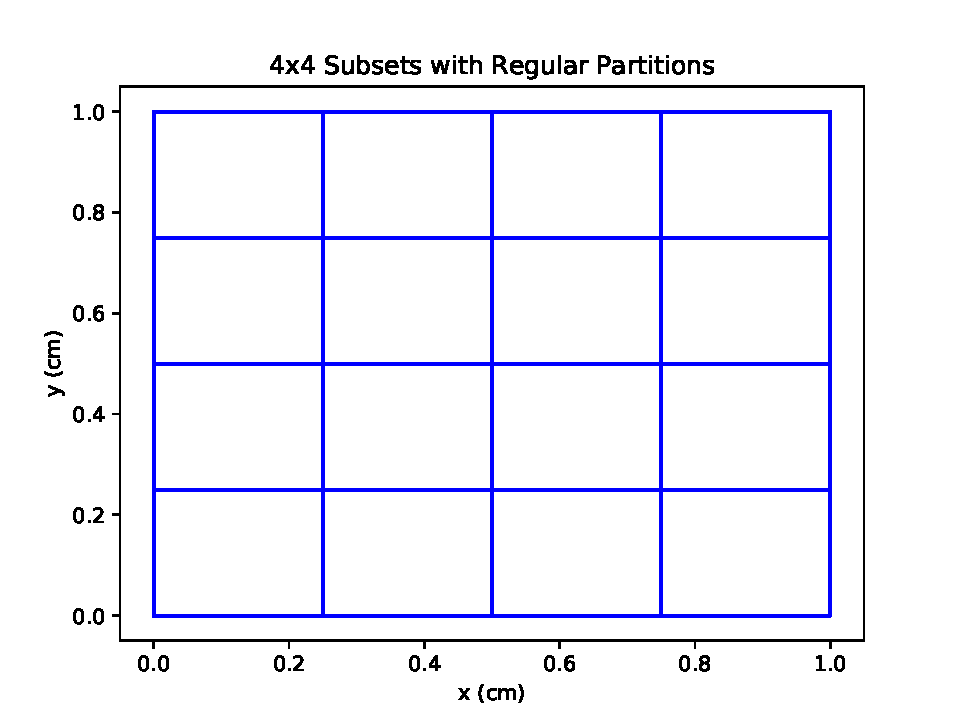
\includegraphics[width=\textwidth]{../cut_line_files/4_regular.pdf}
  \caption{4x4 subsets with regular partitions.}
  \label{4regular}
\end{subfigure}
\begin{subfigure}[b]{0.45\textwidth}
  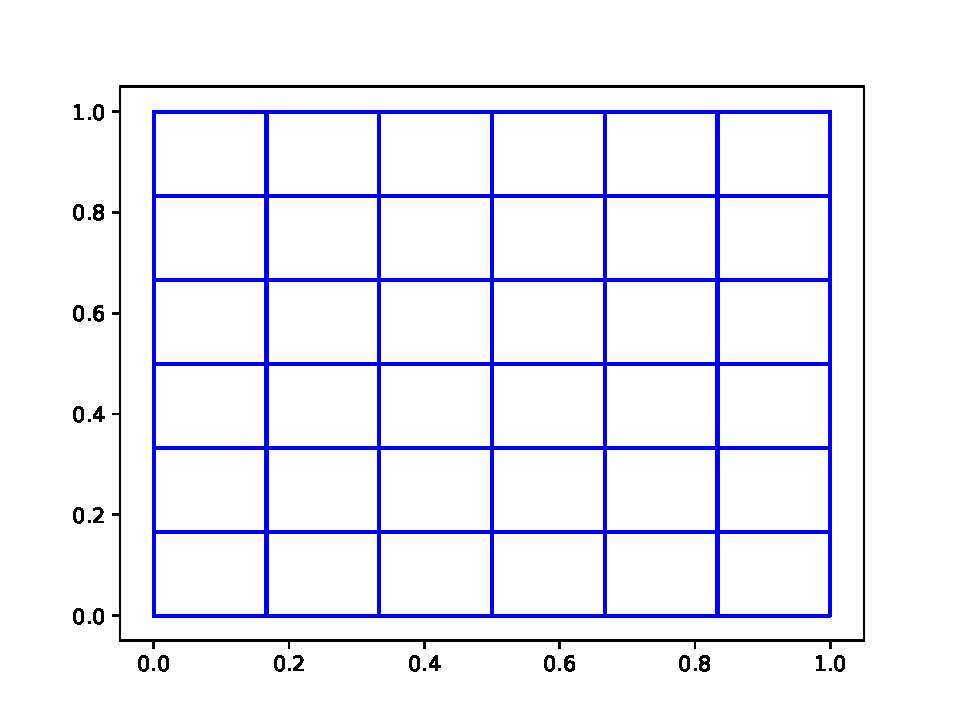
\includegraphics[width=\textwidth]{../cut_line_files/6_regular.pdf}
  \caption{6x6 subsets with regular partitions.}
  \label{6regular}
\end{subfigure}

\begin{subfigure}[b]{0.45\textwidth}
  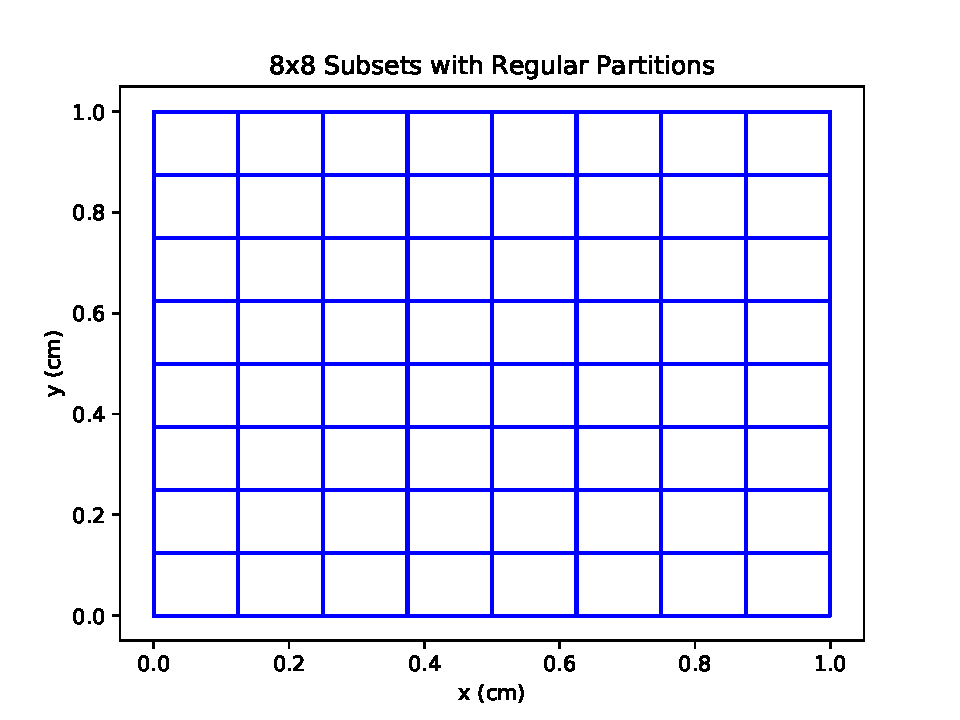
\includegraphics[width=\textwidth]{../cut_line_files/8_regular.pdf}
  \caption{8x8 subsets with regular partitions.}
  \label{8regular}
\end{subfigure}
\begin{subfigure}[b]{0.45\textwidth}
  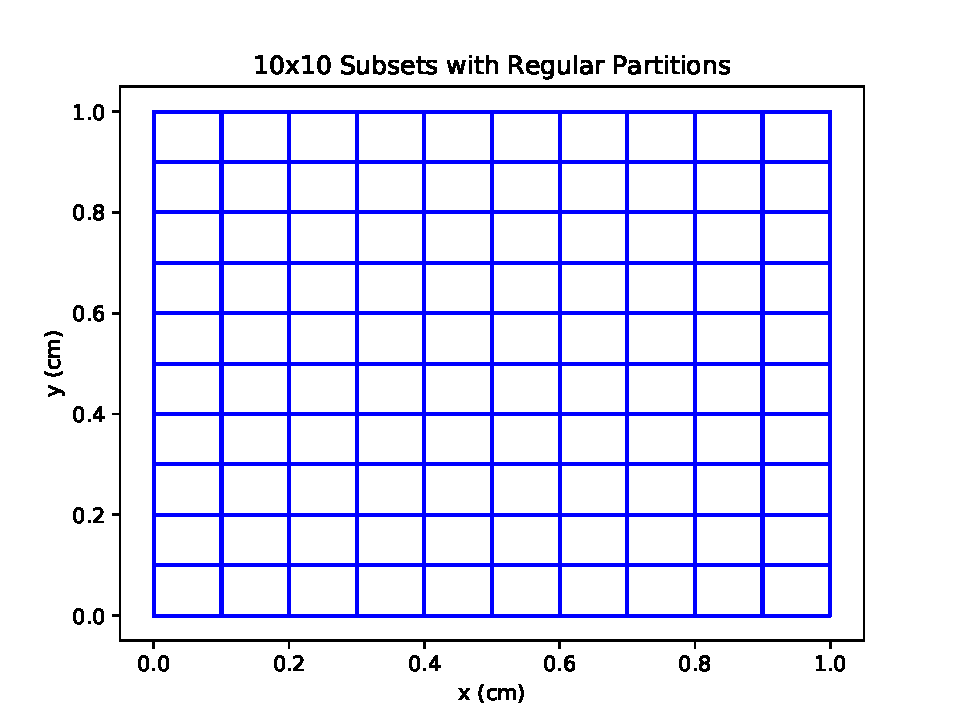
\includegraphics[width=\textwidth]{../cut_line_files/10_regular.pdf}
  \caption{10x10 subsets with regular partitions.}
  \label{10regular}
\end{subfigure}
\caption{Examples of regular partitioning.}
\label{regular_partitions}
\end{figure}

Using regular partitions as shown in Fig.~\ref{regular_partitions}, the first portion of the 2D verification study was run from 2x2 to 10x10 subsets in x and y and 1 to 6 angles per quadrant.  Figure~\ref{regular_verification} shows the results of the time-to-solution estimator (solid line) against Ragusa's code (points) for each test case. The time-to-solution estimator is in perfect agreement for regular partitions with multiple angles per quadrant.

%Verification plots.
\begin{figure}[H]
\centering
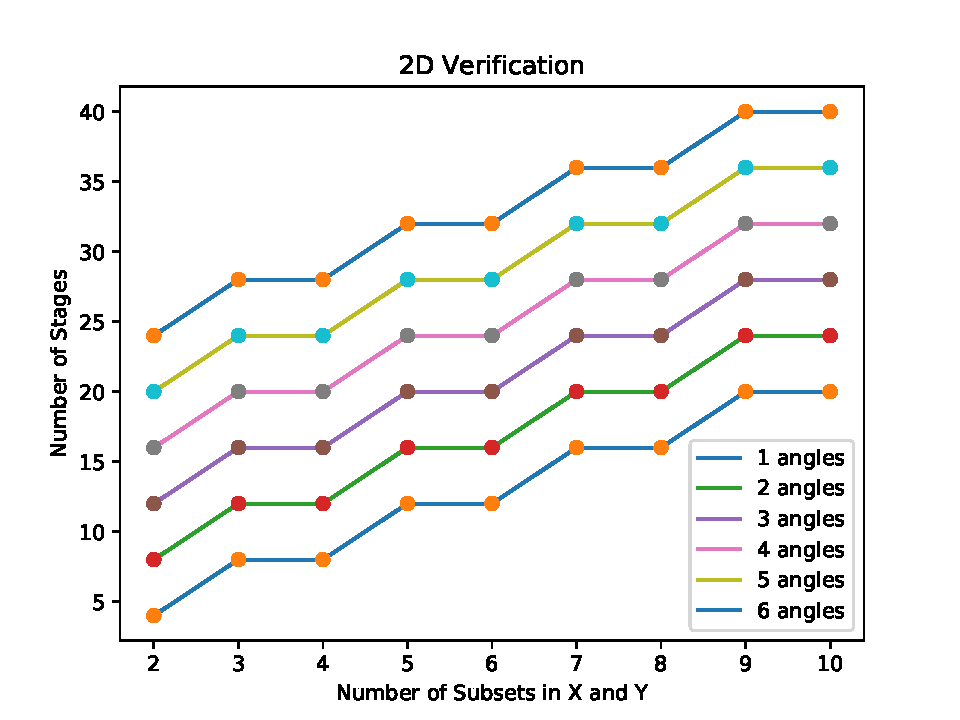
\includegraphics[scale=0.8]{../figures/regular_verification.pdf}
\caption{A 2D verification suite with regular partitions run from 2x2 to 10x10 subsets with each case being run from 1 to 6 anglesets per quadrant.}
\label{regular_verification}
\end{figure}

\subsection{``Mildly Random'' Partitions}
Figure~\ref{mild_random_partitions} shows four examples of the ``mildly random'' partitioning scheme used for the second part of the verification study. Cut lines in the x dimension go all the way across the domain, and are uniformly distributed. This reflects a possible partitioning scheme after the load balancing by dimension algorithm described in Section \ref{sec:lbd} is used.

%Mild random partitions
\begin{figure}[H]
\centering
\begin{subfigure}[b]{0.45\textwidth}
  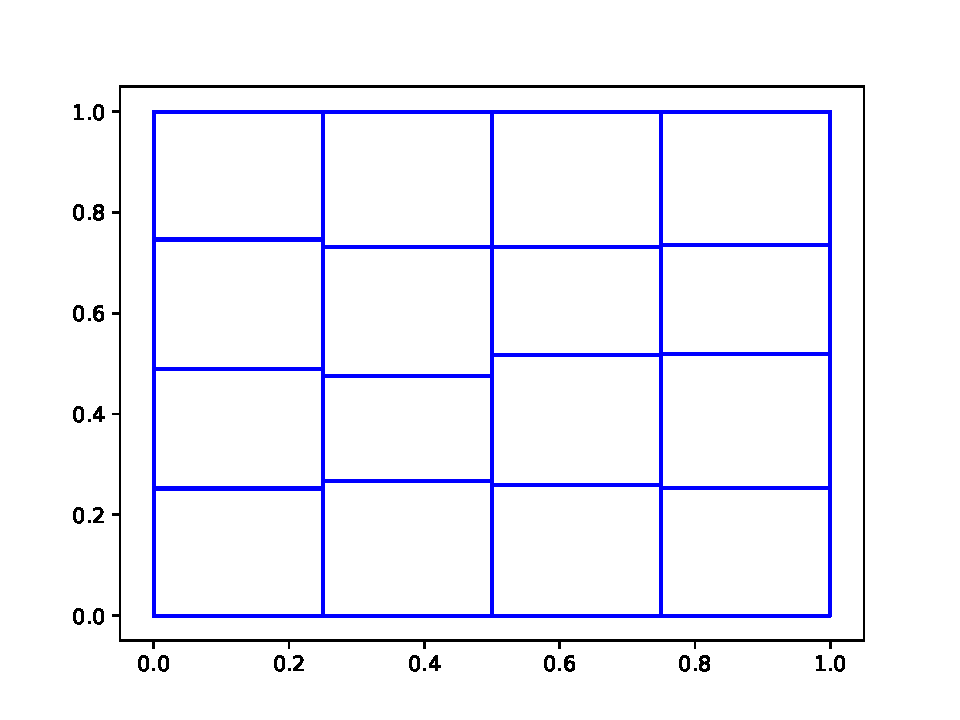
\includegraphics[width=\textwidth]{../cut_line_files/4_mild_random.pdf}
  \caption{4x4 subsets with ``mildly random'' partitions.}
  \label{4mildrandom}
\end{subfigure}
\begin{subfigure}[b]{0.45\textwidth}
  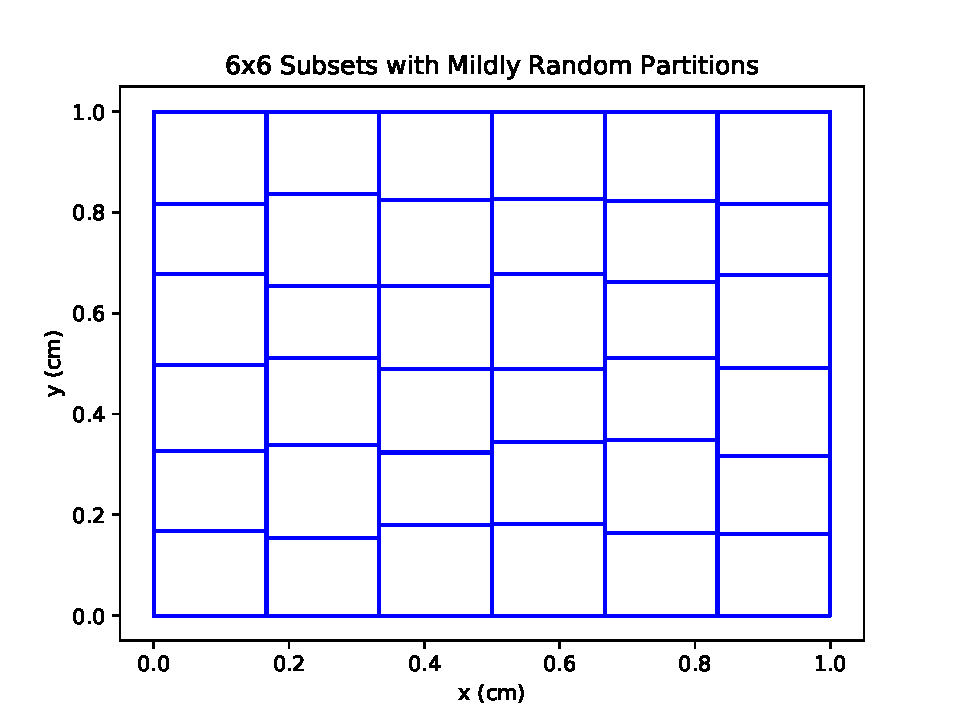
\includegraphics[width=\textwidth]{../cut_line_files/6_mild_random.pdf}
  \caption{6x6 subsets with ``mildly random'' partitions.}
  \label{6mildrandom}
\end{subfigure}

\begin{subfigure}[b]{0.45\textwidth}
  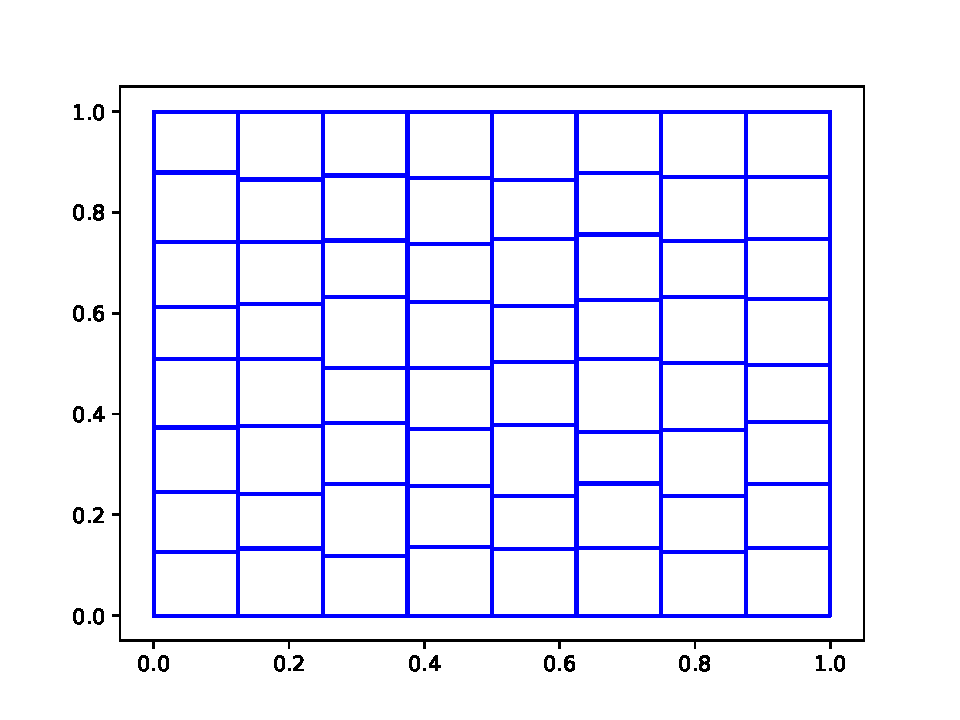
\includegraphics[width=\textwidth]{../cut_line_files/8_mild_random.pdf}
  \caption{8x8 subsets with ``mildly random'' partitions.}
  \label{8mildrandom}
\end{subfigure}
\begin{subfigure}[b]{0.45\textwidth}
  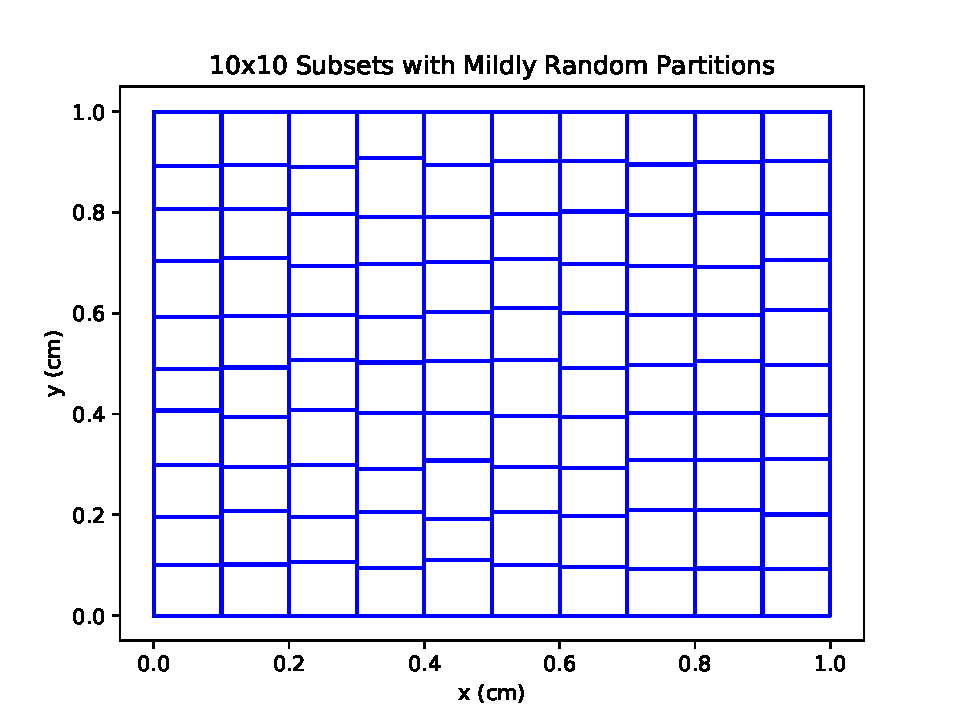
\includegraphics[width=\textwidth]{../cut_line_files/10_mild_random.pdf}
  \caption{10x10 subsets with ``mildly random'' partitions.}
  \label{10mildrandom}
\end{subfigure}
\caption{Examples of ``mildly random'' partitioning.}
\label{mild_random_partitions}
\end{figure}

Using``mildly random'' partitions as shown in Fig.~\ref{mild_random_partitions}, the second portion of the 2D verification study was run from 2x2 to 10x10 subsets in x and y and 1 to 6 angles per quadrant.  Figure~\ref{mild_random_verification} shows the results of the time-to-solution estimator (solid line) against Ragusa's code (points) for each test case. The time-to-solution estimator is in perfect agreement for``mildly random'' partitions with multiple angles per quadrant.

\begin{figure}[H]
\centering
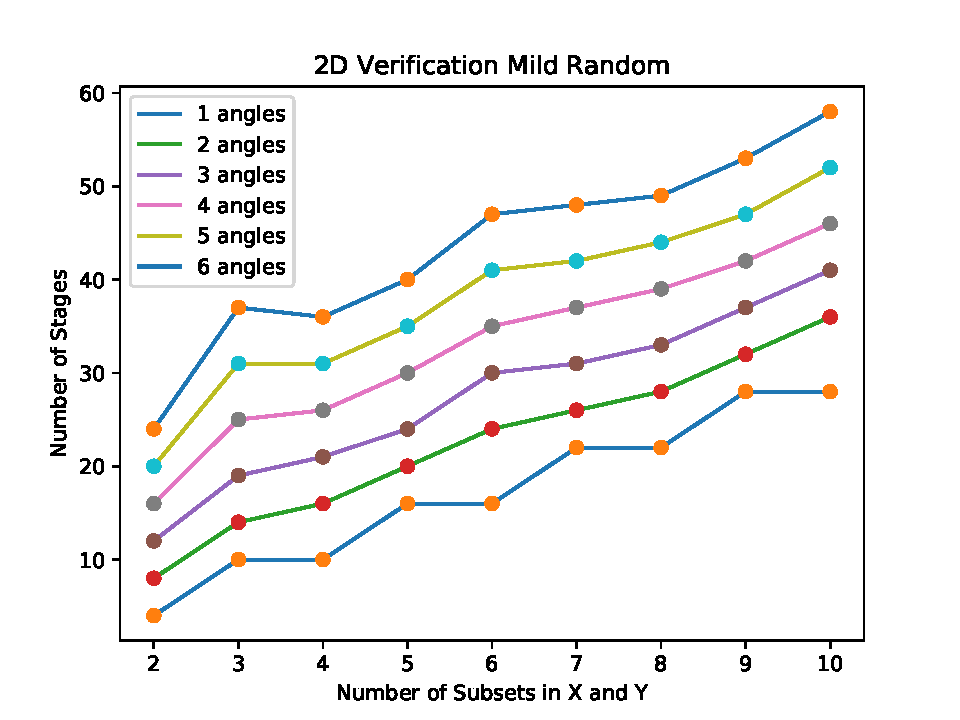
\includegraphics[scale=0.8]{../figures/mild_random_verification.pdf}
\caption{A 2D verification suite with ``mildly random'' partitions run from 2x2 to 10x10 subsets with each case being run from 1 to 6 anglesets per quadrant.}
\label{mild_random_verification}
\end{figure}

\subsection{Random Partitions}
%Random partitions
Figure~\ref{random_partitions} shows four examples of the ``random'' partitioning scheme used for the third part of the verification study. Cut lines in the x dimension go all the way across the domain, but are not necessarily uniformly distributed. The cut lines in y are randomly distributed in each column.This reflects a possible partitioning scheme after the load balancing by dimension algorithm described in Section \ref{sec:lbd} is used.
\begin{figure}[H]
\centering
\begin{subfigure}[b]{0.45\textwidth}
  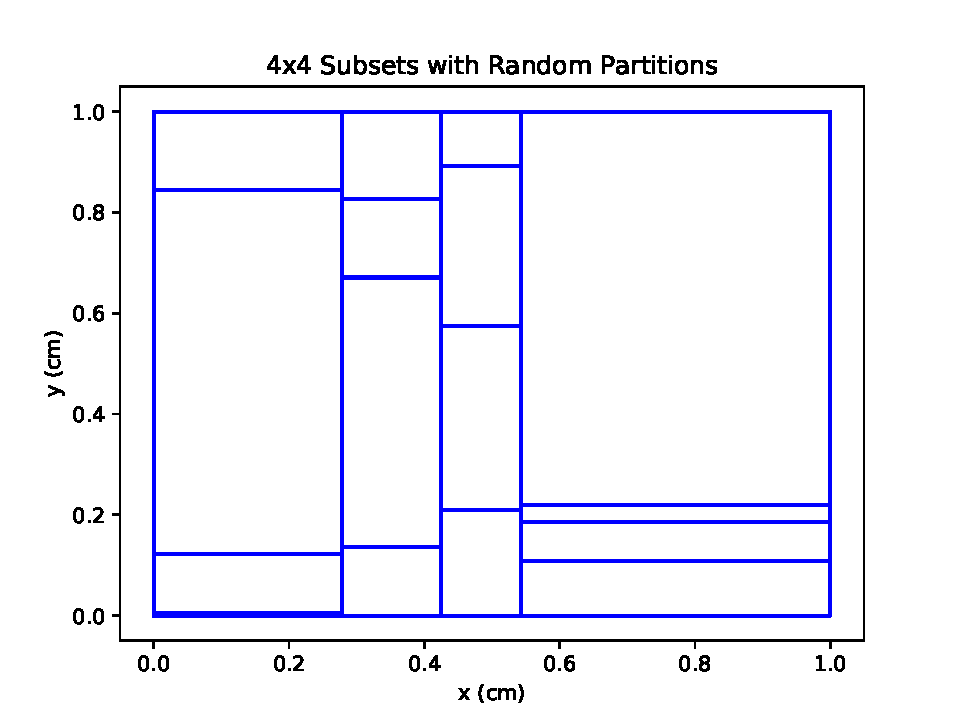
\includegraphics[width=\textwidth]{../cut_line_files/4_random.pdf}
  \caption{4x4 subsets with ``random'' partitions.}
  \label{4random}
\end{subfigure}
\begin{subfigure}[b]{0.45\textwidth}
  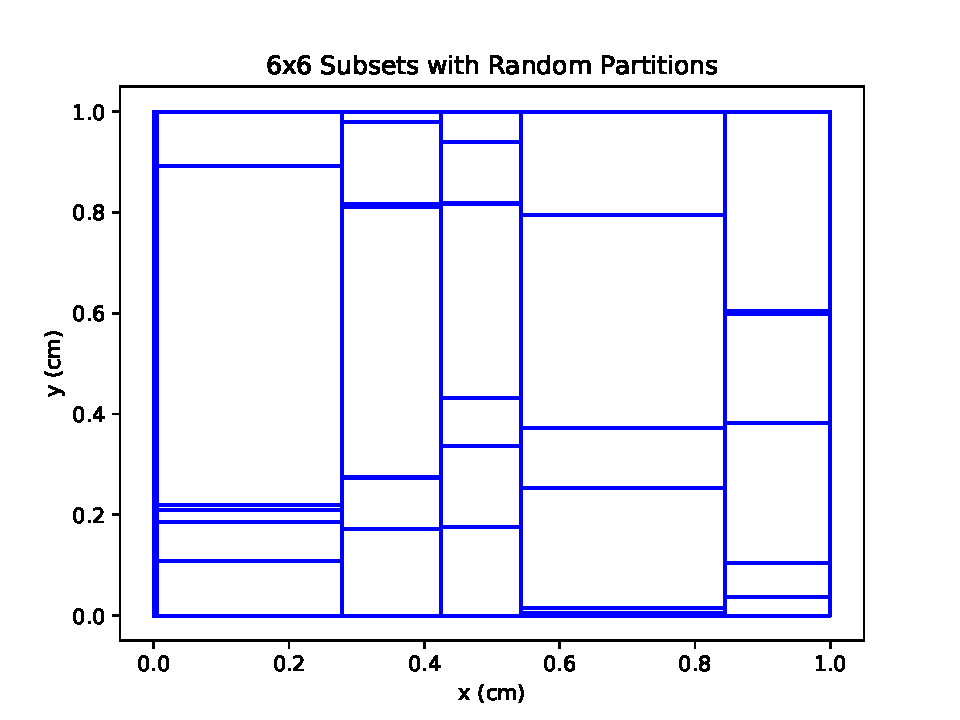
\includegraphics[width=\textwidth]{../cut_line_files/6_random.pdf}
  \caption{6x6 subsets with ``random'' partitions.}
  \label{6random}
\end{subfigure}

\begin{subfigure}[b]{0.45\textwidth}
  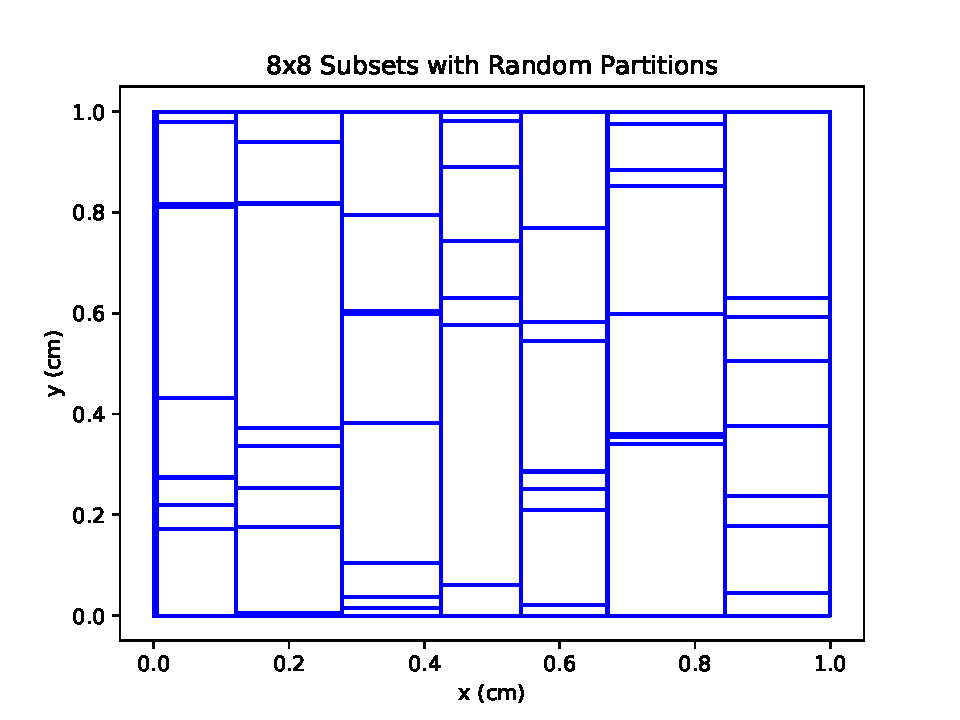
\includegraphics[width=\textwidth]{../cut_line_files/8_random.pdf}
  \caption{8x8 subsets with ``random'' partitions.}
  \label{8random}
\end{subfigure}
\begin{subfigure}[b]{0.45\textwidth}
  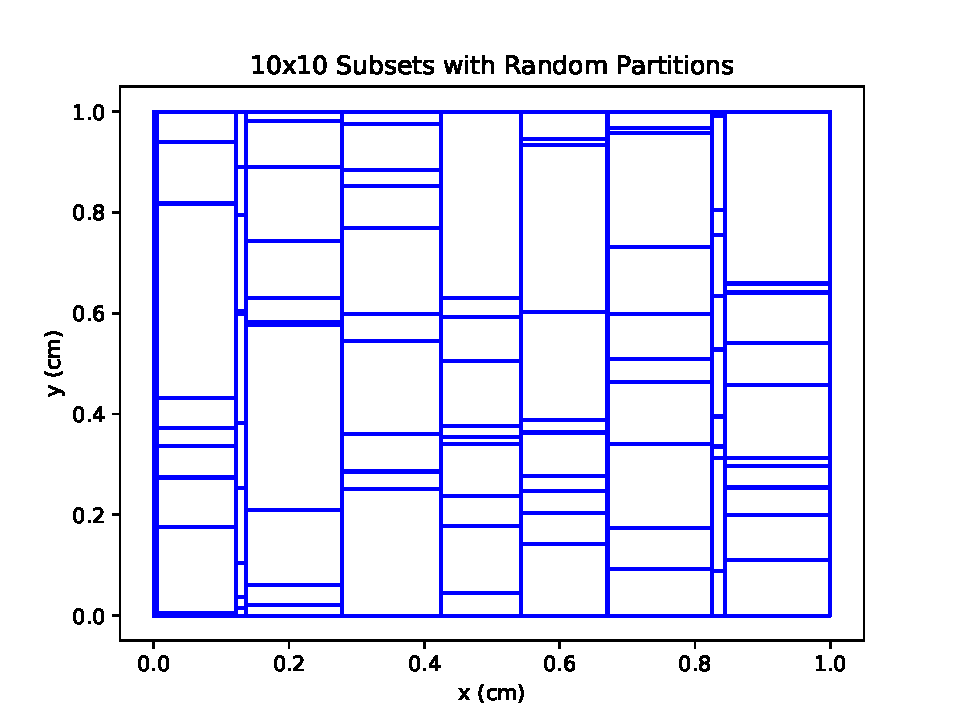
\includegraphics[width=\textwidth]{../cut_line_files/10_random.pdf}
  \caption{10x10 subsets with ``random''partitions.}
  \label{10random}
\end{subfigure}
\caption{Examples of ``random'' partitioning.}
\label{random_partitions}
\end{figure}

Using ``random'' partitions as shown in Fig.~\ref{random_partitions}, the third portion of the 2D verification study was run from 2x2 to 10x10 subsets in x and y and 1 to 6 angles per quadrant.  Figure~\ref{random_verification} shows the results of the time-to-solution estimator (solid line) against Ragusa's code (points) for each test case. The time-to-solution estimator is in perfect agreement for``random''partitions with multiple angles per quadrant.

\begin{figure}[H]
\centering
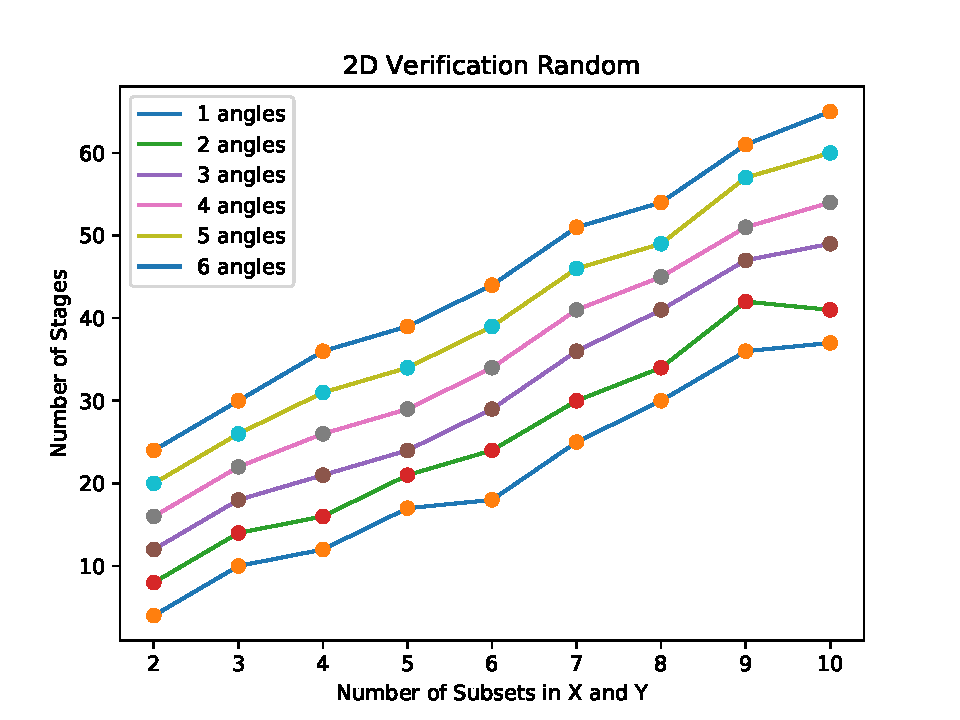
\includegraphics[scale=0.8]{../figures/random_verification.pdf}
\caption{A 2D verification suite with ``random'' partitions run from 2x2 to 10x10 subsets with each case being run from 1 to 6 anglesets per quadrant.}
\label{random_verification}
\end{figure}

\subsection{Probable Worst-Case Partitions}
Figure~\ref{worst_partitions} shows four examples of the probable worst-case partitioning scheme used for the final part of the verification study. Cut lines in the x dimension go all the way across the domain, and are uniformly distributed. The cut lines in y are distributed on opposing ends of alternating columns.This reflects a possible partitioning scheme after the load balancing by dimension algorithm described in Section \ref{sec:lbd} is used.
\begin{figure}[H]
\centering
\begin{subfigure}[b]{0.45\textwidth}
  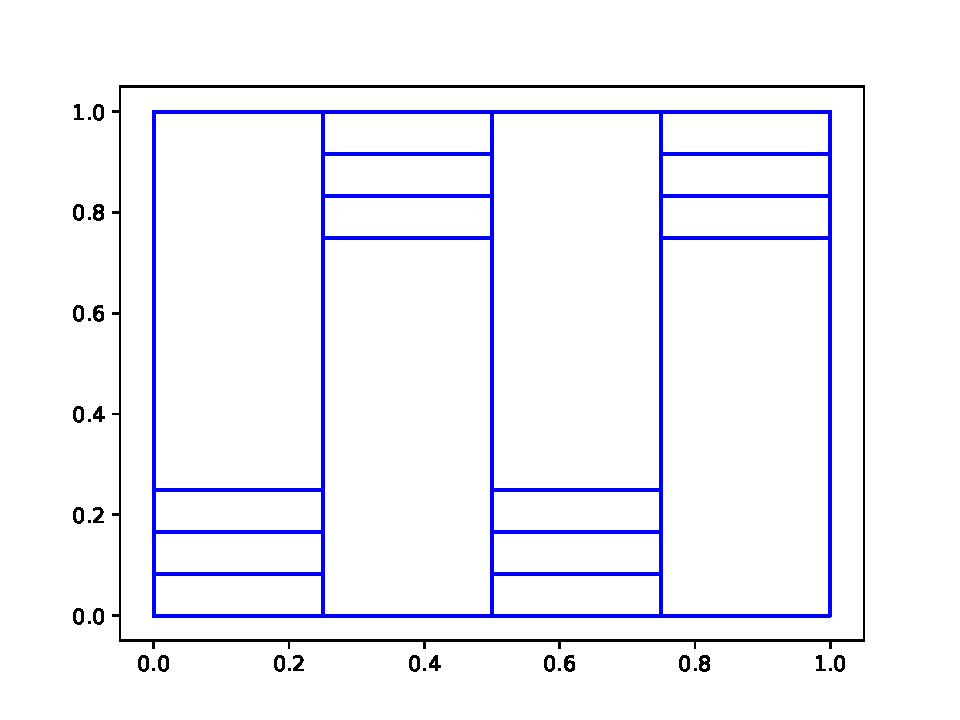
\includegraphics[width=\textwidth]{../cut_line_files/4_worst.pdf}
  \caption{4x4 subsets with probable worst-case partitions.}
  \label{4worst}
\end{subfigure}
\begin{subfigure}[b]{0.45\textwidth}
  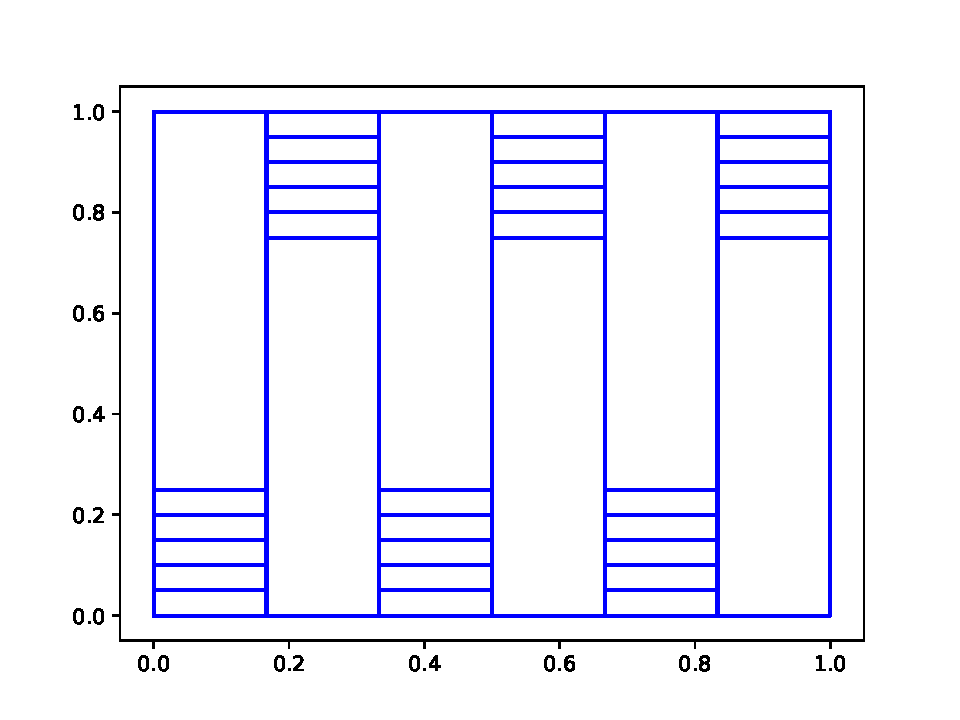
\includegraphics[width=\textwidth]{../cut_line_files/6_worst.pdf}
  \caption{6x6 subsets with probable worst-case partitions.}
  \label{6worst}
\end{subfigure}

\begin{subfigure}[b]{0.45\textwidth}
  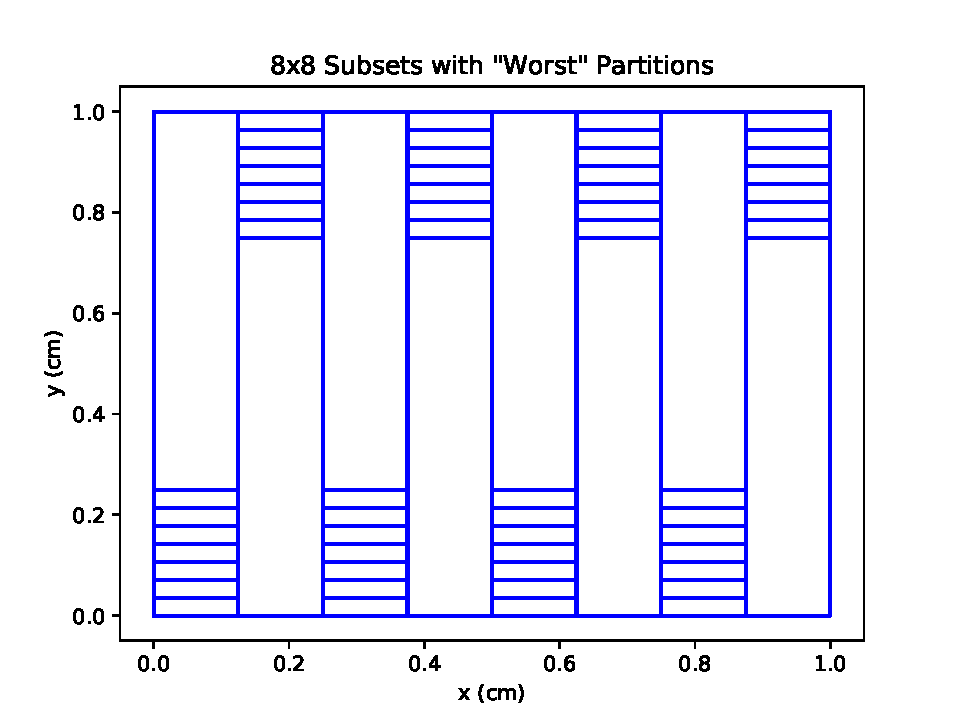
\includegraphics[width=\textwidth]{../cut_line_files/8_worst.pdf}
  \caption{8x8 subsets with probable worst-case partitions.}
  \label{8random}
\end{subfigure}
\begin{subfigure}[b]{0.45\textwidth}
  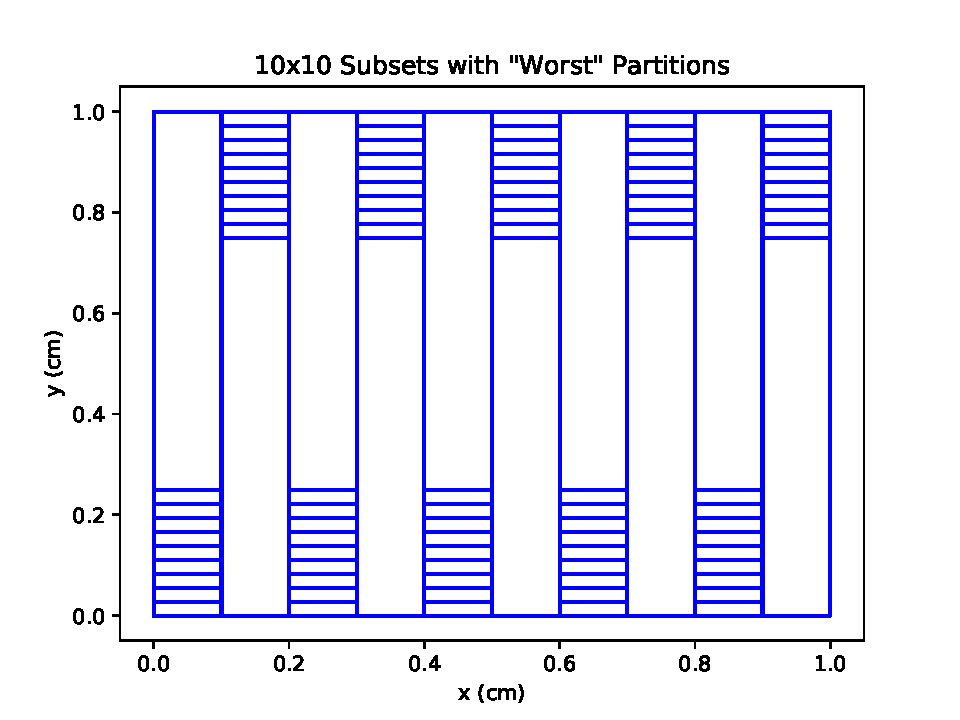
\includegraphics[width=\textwidth]{../cut_line_files/10_worst.pdf}
  \caption{10x10 subsets with probable worst-case partitions.}
  \label{10random}
\end{subfigure}
\caption{Examples of probable worst-case partitioning.}
\label{worst_partitions}
\end{figure}
Using probable worst-case partitions as shown in Fig.~\ref{worst_partitions}, the final portion of the 2D verification study was run from 2x2 to 10x10 subsets in x and y and 1 to 6 angles per quadrant.  Figure~\ref{worst_verification} shows the results of the time-to-solution estimator (solid line) against Ragusa's code (points) for each test case. The time-to-solution estimator is in perfect agreement for probable worst-case partitions with multiple angles per quadrant.
\begin{figure}[H]
\centering
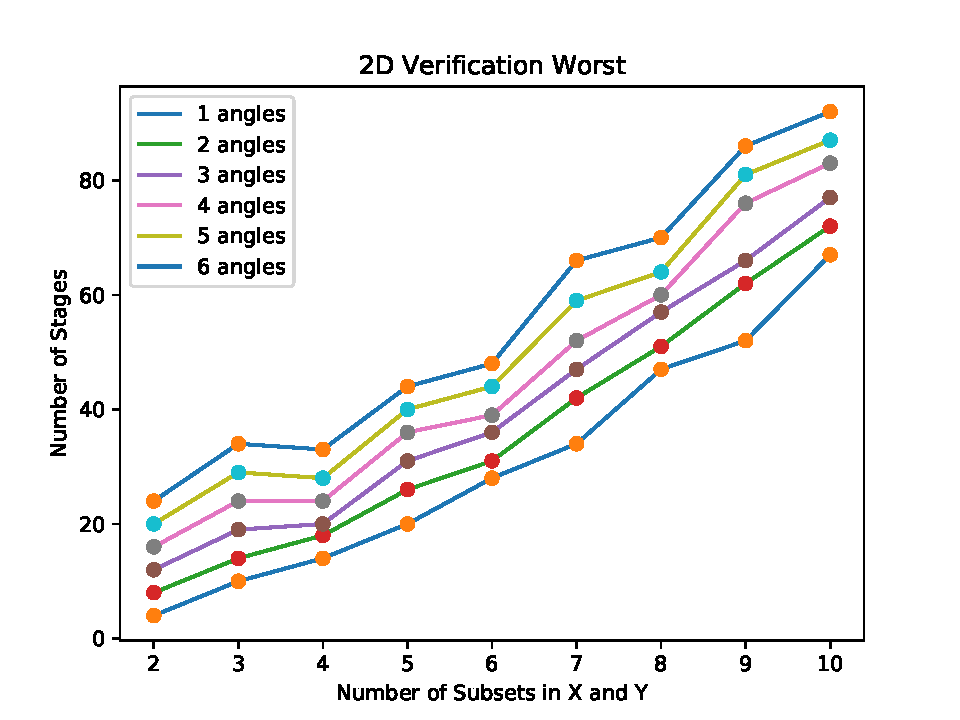
\includegraphics[scale=0.8]{../figures/worst_verification.pdf}
\caption{A 2D verification suite with probable worst-case partitions run from 2x2 to 10x10 subsets with each case being run from 1 to 6 angles per quadrant.}
\label{worst_verification}
\end{figure}

\section{3D Verification}
PDT's performance model is used to verify stage counts for 3D problems with regular grids.
Figure~\ref{3d_verification} shows PDT's performance model stage counts are in perfect agreement with the time-to-solution estimator's stage counts for 2\textsuperscript{3} to 10\textsuperscript{3} subsets and from 1 to 6 angles per octant.

\begin{figure}[H]
\centering
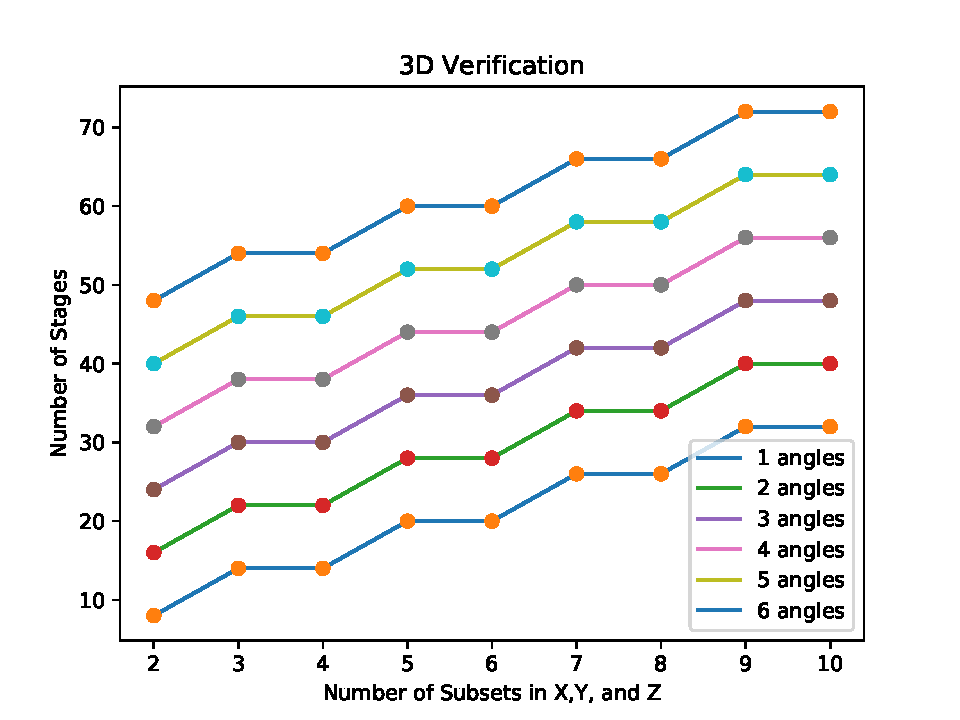
\includegraphics[scale=0.8]{../figures/3d_verification.pdf}
\caption{A 3D verification suite with regular partitions run from 2\textsuperscript{3} to 10\textsuperscript{3} subsets with each case being run from 1 to 6 angles per octant.}
\label{3d_verification}
\end{figure}


\section{PDT's Performance Model vs. Time-to-Solution Estimator}

PDT has run a scaling suite out to 90,112 cores on the Quartz supercomputer \cite{quartz} at Lawrence Livermore National Lab (LLNL).
A smaller scaling suite, tabulated in Table \ref{scaling_suite} is the first benchmark case run for the time-to-solution estimator.
The suite was run with 1 energy group, 80 directions, $A_m = 10$, $A_x=\frac{N_x}{P_x}$, $A_y=\frac{N_y}{P_y}$, and $A_z = 1$.
The following machine parameters were generated and used for the 1 group suite:
\begin{itemize}
  \item $T_c = 2683.769$ ns
  \item $T_m = 111.972$ ns
  \item $T_g = 559.127$ ns
  \item $T_\text{byte} = 4.47$ ns
  \item $\text{latency }= 4110$ ns
  \item $M_L = 2.5$
  \item $T_{wu} = 5779.929$ ns
  \item mcff = 1.32
\end{itemize}

\begin{table}[H]
  \centering
  \caption{The scaling suite parameters ran with 1 energy group, 80 directions, and $A_m = 10$.}
  \label{scaling_suite}
  \begin{tabular}{c|c|c|c|c|c|c|c|c|c}
    \textbf{Cores} & 1 & 8 & 64 & 512 & 1,204 & 2,048 & 4,096 & 8,192 & 16,384 \\ \hline
    \textbf{Nx} & 16 & 32 & 64 & 128 & 128 & 256 & 256 & 256 & 512 \\ \hline
    \textbf{Ny} & 16 & 32 & 64 & 128 & 128 & 128 & 128 & 256 & 256 \\ \hline
    \textbf{Nz} & 16 & 32 & 64 & 128 & 256 & 256 & 256 & 512 & 512 \\ \hline
    \textbf{Px} & 1  & 2  & 8  & 16  & 32  & 32  & 64  & 64  & 128 \\ \hline
    \textbf{Py} & 1  & 2  & 4  & 16  & 16  & 32  & 32  & 64  & 64  \\ \hline
    \textbf{Pz} & 1  & 2  & 2  & 2   & 2   & 2   & 2   & 2   & 2   \\
  \end{tabular}
\end{table}

Figure~\ref{scaling_stagecount} shows the stage counts of the scaling suite for PDT's performance model and the time-to-solution estimator are in perfect agreement.
Figures \ref{weak_scaling_tts_sweep} and \ref{weak_scaling_tts} show the time per sweep and parallel efficiency for (1) PDT, (2) the PDT performance model, and (3) the time-to-solution estimator. Table \ref{scaling_percent_diff} tabulates the percent differences for (1) PDT and the performance model, (2) the performance model, and (3) the time-to-solution estimator, and PDT and the time-to-solution estimator.

It is noteable that the time-to-solution estimator consistently returns a smaller sweep time value than PDT's performance model. This is certainly in part due to the assumption from PDT's performance model that each processors at each stage communicate to the same amount of neighbors (three neighbors in 3D, 2 in 2D).
In reality, this is not the case, as processors in the corners of the domain will communicate to fewer neighbors for certain directions, and the final processor for a direction does not communicate to any neighbors (as it has no successors).
Because the stage counts for the performance model and time-to-solution estimator are in perfect agreement (as shown in Fig.~\ref{scaling_stagecount}), we know that this slight overestimation of the performance model is a reason for its consistently higher sweep times.
Even given these differences, the time-to-solution estimator is consistently within 4\% of the performance model, as tabulated in Table \ref{scaling_percent_diff}.

The performance model's slightly better accuracy in predicting PDT's sweep time is likely due to processor noise and slight variations in latency on Quartz driving up PDT's sweep time. This masks the performance model's slight overestimation of the sweep time.

Figure~\ref{weak_scaling_tts} shows PDT's performance model and the time-to-solution estimator scale with near equivalence. The model and the time-to-solution estimator predict PDT's scaling well, although there are slight differences that can be attributed to the differences in sweep times tabulated in Table \ref{scaling_percent_diff}.
\begin{figure}[ht]
\centering
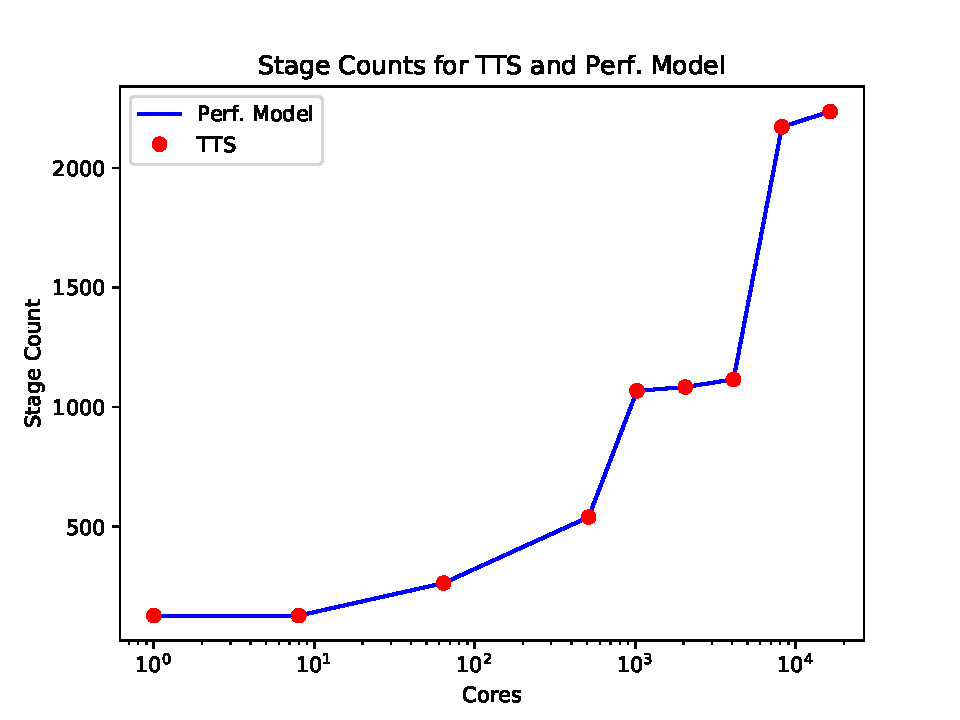
\includegraphics[scale=0.8]{../../figures/scaling_stagecount.pdf}
\caption{The stage counts of PDT's performance model and the time-to-solution estimator for the scaling suite in Table \ref{scaling_suite}.}
\label{scaling_stagecount}
\end{figure}
\begin{figure}[ht]
\centering
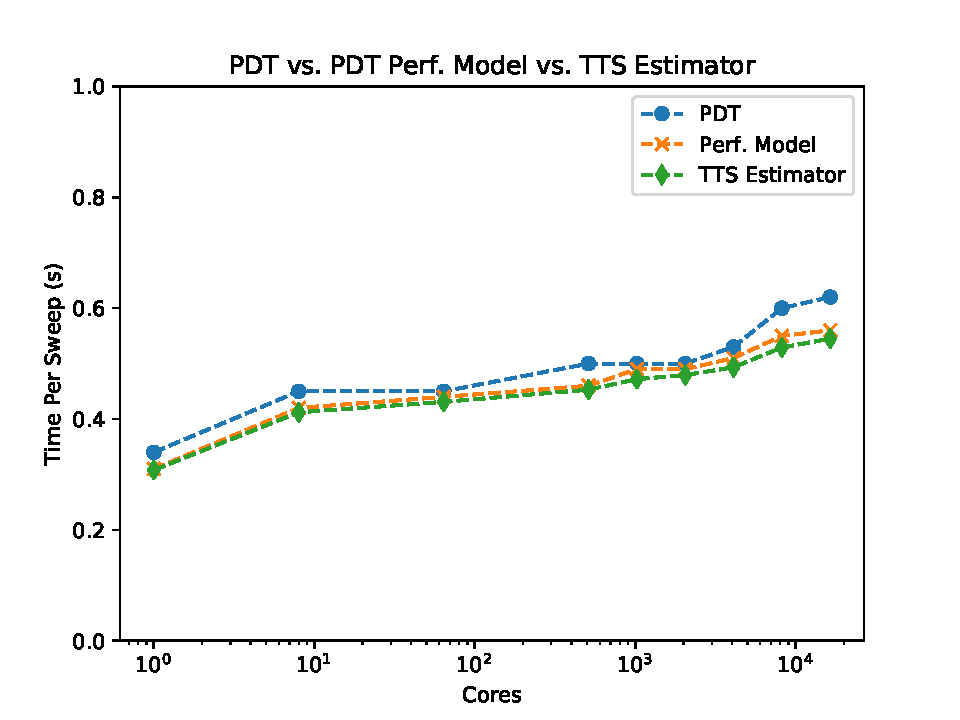
\includegraphics[scale=0.8]{../../figures/scaling_tts_sweep_times.pdf}
\caption{The time per sweep of PDT, the PDT performance model, and the time-to-solution estimator.}
\label{weak_scaling_tts_sweep}
\end{figure}
\begin{figure}[ht]
\centering
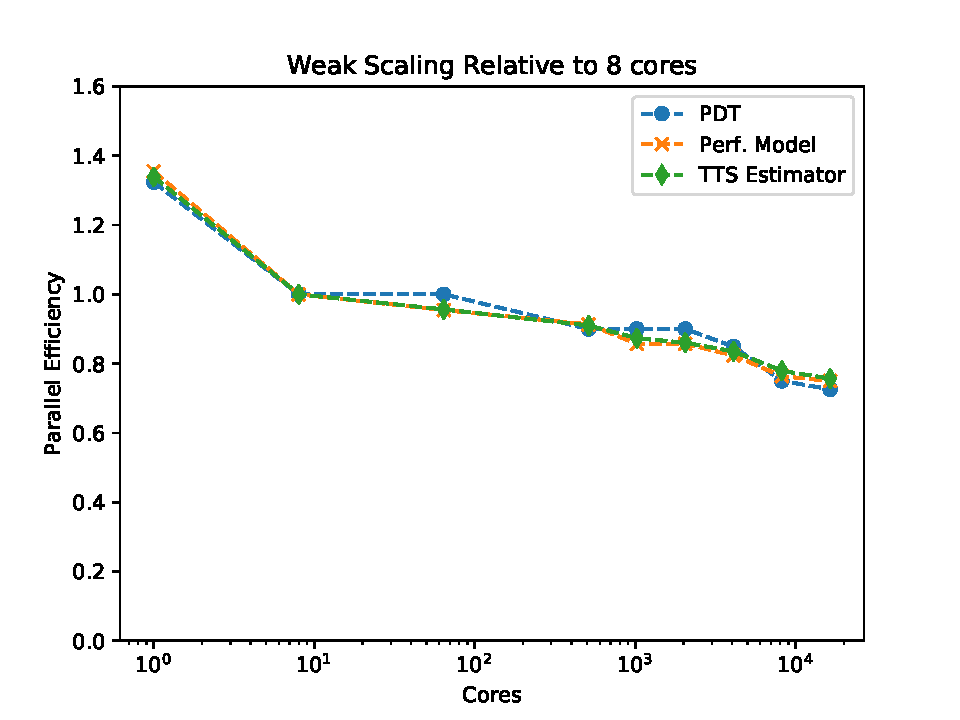
\includegraphics[scale=0.8]{../../figures/scaling_tts.pdf}
\caption{The parallel efficiency relative to 8 cores of PDT, the PDT performance model, and the time-to-solution estimator.}
\label{weak_scaling_tts}
\end{figure}
\begin{table}[ht]
\centering
\caption{The percent difference between (1) PDT and its performance model, (2) PDT's performance model and the time-to-solution estimator, and (3) PDT and the time-to-solution estimator.}
\label{scaling_percent_diff}
\begin{tabular}{c|c|c|c}
\textbf{Cores} & \textbf{PDT v. Perf.} & \textbf{Perf. v. TTS} & \textbf{PDT v. TTS} \\ \hline
1&8.82\%&0.68\%&9.44\% \\ \hline
8&6.67\%&1.86\%&8.4\% \\ \hline
64&2.22\%&2.04\%&4.22\% \\ \hline
512&8.0\%&1.52\%&9.4\% \\ \hline
1024&2.0\%&3.67\%&5.6\% \\ \hline
2048&2.0\%&2.21\%&4.17\% \\ \hline
4096&3.77\%&3.24\%&6.89\% \\ \hline
8192&8.33\%&3.8\%&11.82\% \\ \hline
16384&9.68\%&2.7\%&12.11\%
\end{tabular}
\end{table}

\section{PDT vs. Time-to-Solution Estimator for Unstructured Meshes}

The motivation to develop the time-to-solution estimator was born out of the desire to predict sweep time for unstructured meshes.
To test how the time-to-solution estimator performs on unstructured problems, we use the meshes from our load balancing parametric study: the unbalanced pin mesh(Fig. \ref{partitioning_example}) and the Level-2 experiment mesh (Fig. \ref{level2_nocut_lbchapter}).

All problems were run with one energy group, one subset per processor, and 144 angles with $A_m = 36$, or 36 angles per angleset. The machine parameters used for all problems are:
\begin{itemize}
  \item $T_c = 1208.383$ ns
  \item $T_m = 65.54614$ ns
  \item $T_g = 175.0272$ ns
  \item $T_\text{byte} = 4.47$ ns
  \item $\text{latency }= 4110$ ns
  \item $T_{wu} = 147.0754$ ns
  \item mcff = 1.181
\end{itemize}

For each result presented, the problem is run through PDT 10 times on the Quartz supercomputer.
This allows us to filter out outlying values due to supercomputer noise by taking the median solve time per sweep for each problem.
For each result in PDT, the median sweep time value, the maximum sweep time value, and the minimum sweep time value are plotted to showcase the outlying values that can occur.
In order to minimize the effects of the sweep overhead on the timing statistics, the solve time per sweep is calculated from the mean time of ten transport sweeps for each case.

\subsection{PDT vs. the Time-to-Solution Estimator for the Unbalanced Pin Mesh}
Figure~\ref{comp_reg_spiderweb} shows the sweep times for PDT and the time-to-solution estimator for the unbalanced pin mesh with 2 to 10 subsets in each dimension with regular cuts.
Table \ref{diff_reg_spiderweb} tabulates the percent difference between PDT and the time-to-solution estimator for each of the regular test cases run.
We notice that there is better agreement for cases where there are more unknowns.
These cases for the the unbalanced pin mesh with regular cuts are cases with 3, 4, 6, 7, 8, and 9 subsets in each dimension, with cut lines cutting through cells and increasing the total number of cells throughout the mesh.
Cases with 2, 5, and 10 subsets in each dimension have cuts coinciding with natural boundaries, adding no unknowns to the mesh.
More unknowns lead to better timing statistics for PDT, increasing the likelihood of agreement with the time-to-solution estimator.
%spiderweb comp for reg
\begin{figure}[!ht]
\centering
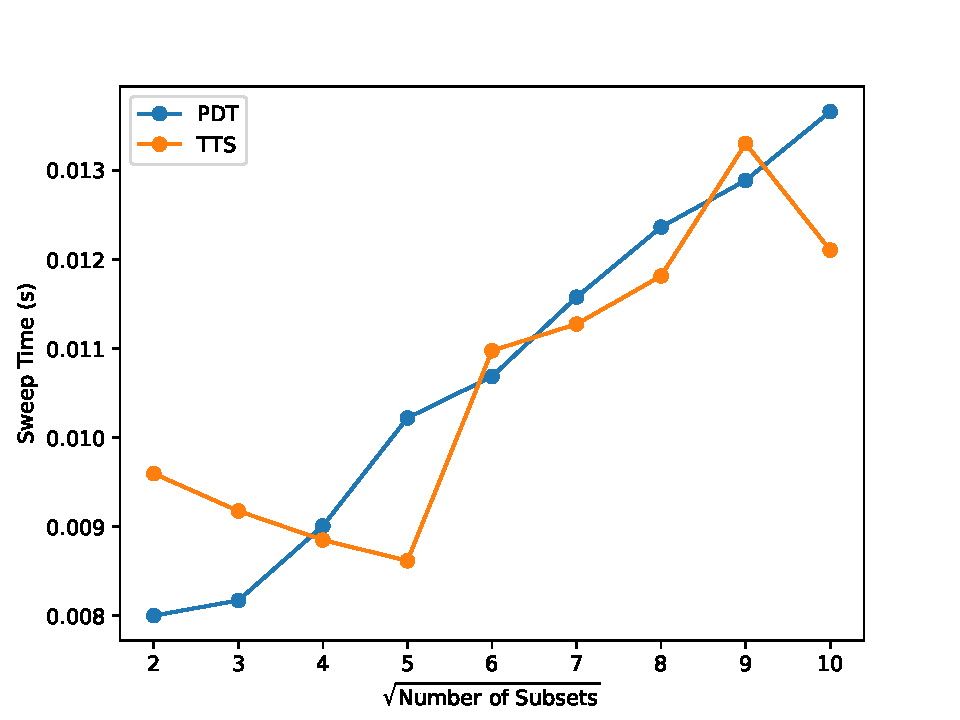
\includegraphics[scale=0.75]{../../figures/spiderweb_reg_pdtvtts.pdf}
\caption{The sweep times of the time-to-solution estimator and PDT for the unbalanced pin mesh for 2 to 10 subsets in each dimension with regular cuts.}
\label{comp_reg_spiderweb}
\end{figure}
\begin{table}[!ht]
\centering
\caption{The percent difference in sweep times between the time-to-solution estimator and PDT for the sweep times shown in Fig.~\ref{comp_reg_spiderweb}.}
\label{diff_reg_spiderweb}
\begin{tabular}{c|c}
\textbf{$\sqrt{\text{Num Subsets}}$} & \bf PDT vs. TTS \\ \hline
2&19.93\%\\ \hline
3&12.3\%\\ \hline
4&1.75\%\\ \hline
5&15.69\%\\ \hline
6&2.71\%\\ \hline
7&2.61\%\\ \hline
8&4.45\%\\ \hline
9&3.21\%\\ \hline
10&11.38\%
\end{tabular}
\end{table}

Figure~\ref{comp_lb_spiderweb} shows the sweep times for PDT and the time-to-solution estimator for 2 to 10 subsets in each dimension with load-balanced cuts.
If we focus on the maximum PDT sweep time in the 5 subset case in Fig.~\ref{comp_lb_spiderweb}, we can see that PDT can sometimes produce outliers during runs.
For that reason, we take the median, not the mean, sweep time value from the ten PDT runs to get the best representation of PDT's solve time per sweep.
Table \ref{diff_lb_spiderweb} tabulates the percent difference between PDT and the time-to-solution estimator for each case run.
We notice that we have poorer agreement with load-balanced cuts than with regular cuts, particularly for lower subset cases.
This is possibly due to the first-come-first scheduler in PDT and the schedule of the time-to-solution estimator schedule not being in perfect agreement.
While the time-to-solution estimator's schedule is deterministic, there are no guarantees that PDT's first-come-first-serve schedule is repeatable or that it matches the time-to-solution estimator.
If there are two tasks that have a similar amount of unknowns, the processor with more unknowns may solve and communicate them faster than the processor with less unknowns.
This would cause a disagreement between the time-to-solution estimator and PDT.
The low subset cases happen to be the more balanced cases for the unbalanced pin mesh with load-balanced cuts.
The 2, 3, and 4 subset cases for the unbalanced pin mesh have load-balance metric values of $f = 1.76, 2.58,$ and $2.38$ respectively.
With a more even distribution of cells, PDT's first-come-first-serve schedule is likelier to deviate more as certain processors may be faster than their neighboring processors.
%spiderweb comp for lb
\begin{figure}[!ht]
  \centering
  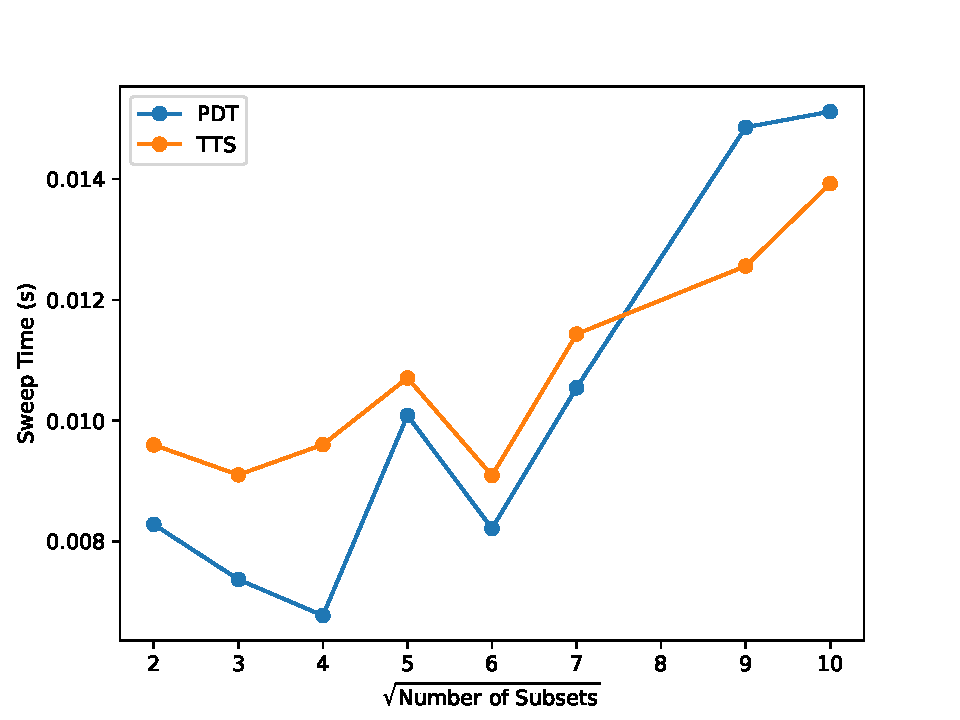
\includegraphics[scale=0.75]{../../figures/spiderweb_lb_pdtvtts.pdf}
  \caption{The sweep times of the time-to-solution estimator and PDT for the mesh in Fig.~\ref{partitioning_example} for 2 to 10 subsets in each dimension with load-balanced cuts.}
\label{comp_lb_spiderweb}
\end{figure}
\begin{table}[!ht]
\centering
\caption{The percent difference in sweep times between the time-to-solution estimator and PDT for the sweep times shown in Fig.~\ref{comp_lb_spiderweb}.}
\label{diff_lb_spiderweb}
\begin{tabular}{c|c}
\textbf{$\sqrt{\text{Num Subsets}}$} & \bf PDT vs. TTS \\ \hline
2&15.9\%\\ \hline
3&23.52\%\\ \hline
4&41.83\%\\ \hline
5&6.15\%\\ \hline
6&10.67\%\\ \hline
7&8.43\%\\ \hline
9&15.47\%\\ \hline
10&7.88\%
\end{tabular}
\end{table}

Figure~\ref{comp_lbd_spiderweb} shows the sweep times for PDT and the time-to-solution estimator for 2 to 10 subsets in each dimension with load-balanced-by-dimension cuts.
Table \ref{diff_lbd_spiderweb} tabulates the percent difference between PDT and the time-to-solution estimator for each case run.
The load-balanced-by-dimension cases for the unbalanced pin mesh have more consistent agreement than the regular cut and load-balanced cut cases.
With load balancing by dimension, more cells are consistently created by slicing through cells in order to get more balanced partitions.
By increasing the number of unknowns, we get better timing statistics for the solve time per sweep.
In addition, with load-balanced-by-dimension partitions, PDT's first-come-first-serve scheduler is more likely to agree with the time-to-solution estimator's.
The communication dependencies inherently created by load-balanced-by-dimension partitions mitigate the likelihood of faster processors disrupting the expected schedule, as seen with the load-balanced cases.
%%%spiderweb comp for lbd
\begin{figure}[!ht]
  \centering
  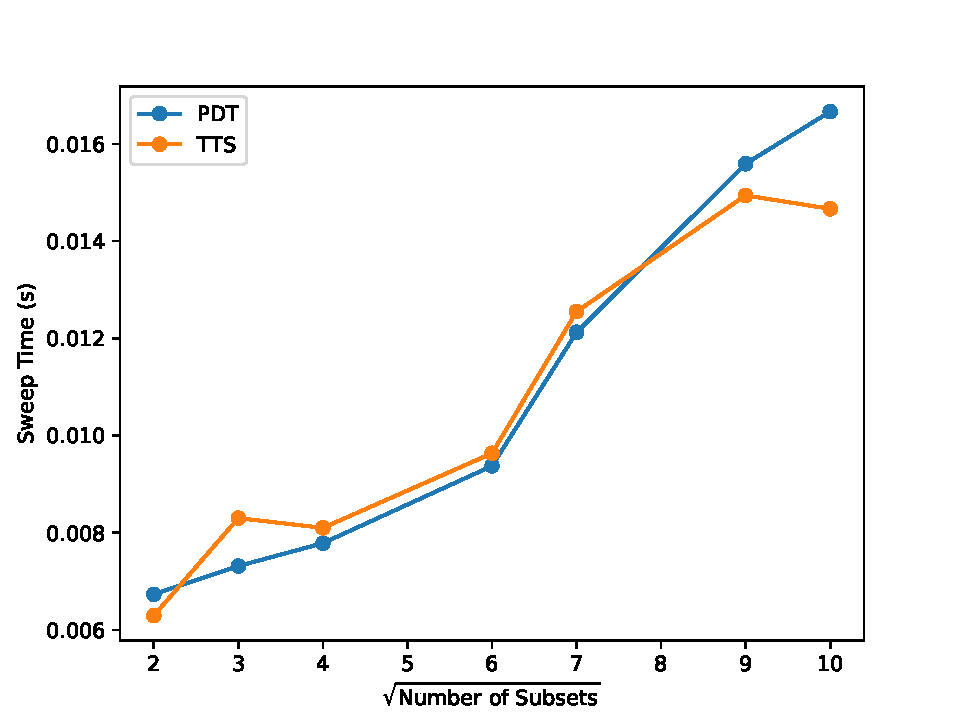
\includegraphics[scale=0.75]{../../figures/spiderweb_lbd_pdtvtts.pdf}
  \caption{The sweep times of the time-to-solution estimator and PDT for the mesh in Fig.~\ref{partitioning_example} for 2 to 10 subsets in each dimension with load-balanced-by-dimension cuts.}
\label{comp_lbd_spiderweb}
\end{figure}
\begin{table}[!ht]
\centering
\caption{The percent difference in sweep times between the time-to-solution estimator and PDT for the sweep times shown in Fig.~\ref{comp_lbd_spiderweb}.}
\label{diff_lbd_spiderweb}
\begin{tabular}{c|c}
\textbf{$\sqrt{\text{Num Subsets}}$} & \bf PDT vs. TTS \\ \hline
2&6.5\%\\ \hline
3&13.49\%\\ \hline
4&4.04\%\\ \hline
6&2.78\%\\ \hline
7&3.5\%\\ \hline
9&4.18\%\\ \hline
10&12.01\%
\end{tabular}
\end{table}

\FloatBarrier
Figure~\ref{ubp_more_sparse} shows a more refined version of the unbalanced pin mesh, containing 9656 cells as opposed to 420 cells. 
Figure~\ref{comp_reg_sparse} shows the sweep times for PDT and the time-to-solution estimator for the unbalanced pin mesh with 2 to 10 subsets in each dimension with regular cuts.
Table \ref{diff_reg_sparse} tabulates the percent difference between PDT and the time-to-solution estimator for each of the regular test cases run.
%%%%
\begin{figure}[H]
\centering
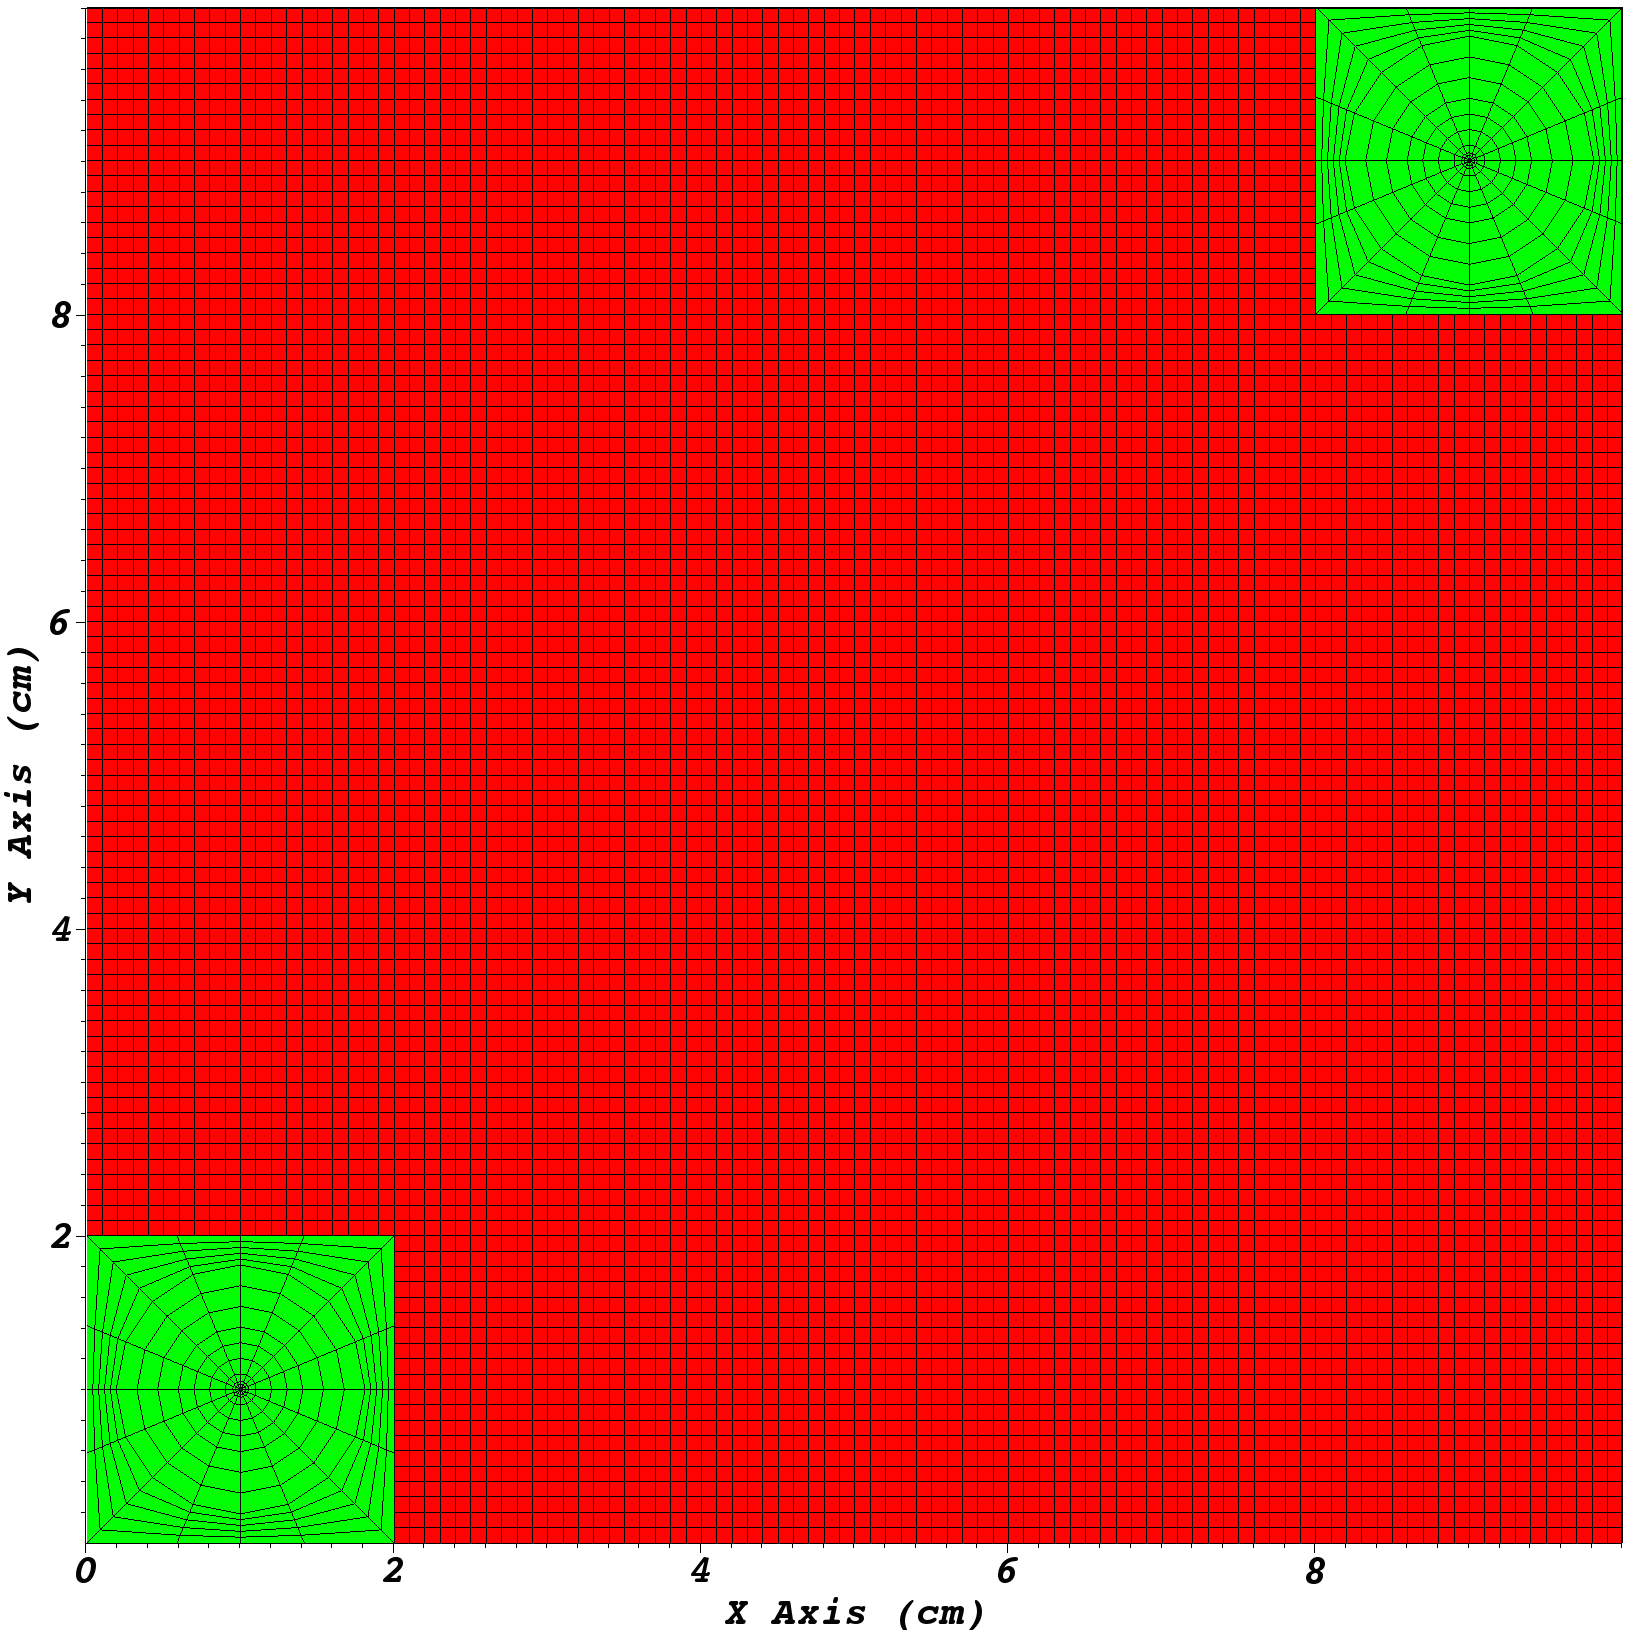
\includegraphics[scale=0.28]{../../figures/unbalanced_pins_more_sparse.png}
\caption{A more refined version of the unbalanced pin mesh, containing 9656 cells as opposed to 420 cells.}
\label{ubp_more_sparse}
\end{figure}
%%%
\begin{figure}[h]
\centering
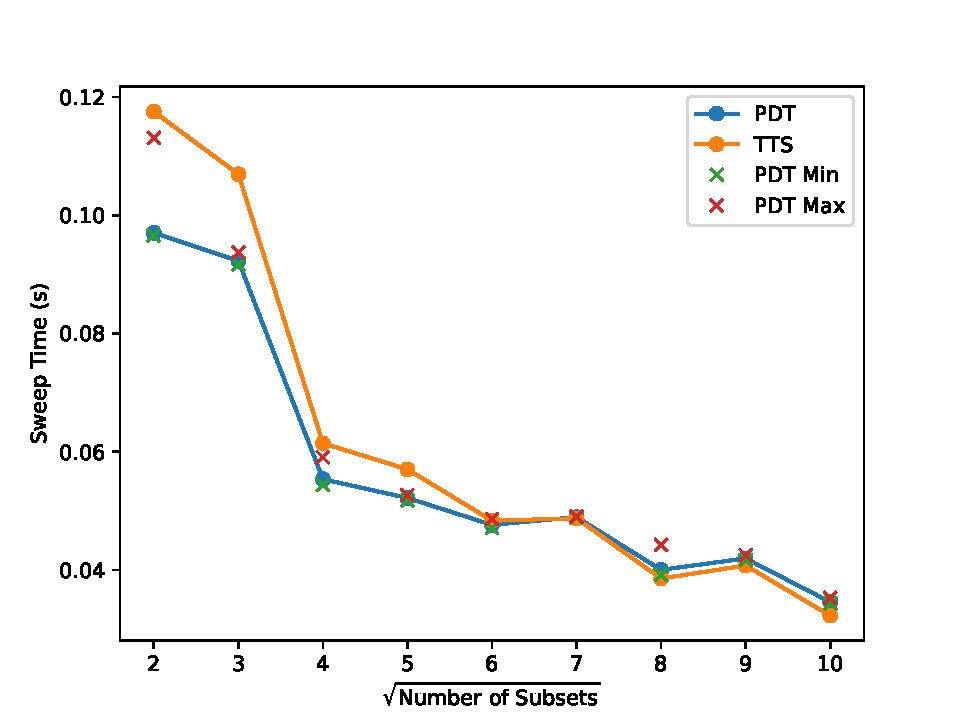
\includegraphics{../../figures/more_sparse_reg_pdtvtts.pdf}
\caption{The sweep times of the time-to-solution estimator and PDT for the more refined unbalanced pin mesh for 2 to 10 subsets in each dimension with regular cuts}
\label{comp_reg_sparse}
\end{figure}
%%%
\begin{table}[h]
\centering
\caption{The percent difference in sweep times between the time-to-solution estimator and PDT for the sweep times shown in Fig.~\ref{comp_reg_sparse}.}
\label{diff_reg_sparse}
\begin{tabular}{c|c}
\textbf{$\sqrt{\text{Num Subsets}}$} & \bf PDT vs. TTS \\ \hline 
2&21.14\%\\ \hline 
3&15.87\%\\ \hline 
4&10.96\%\\ \hline 
5&9.3\%\\ \hline 
6&1.47\%\\ \hline 
7&0.41\%\\ \hline 
8&3.68\%\\ \hline 
9&2.85\%\\ \hline 
10&6.62\%
\end{tabular}
\end{table}

The 9656 cell unbalanced pin mesh time-to-solution estimator sweep times show more consistent agreement with PDT than the 420 cell unbalanced pin mesh.
In addition, the behaviors of PDT and the time-to-solution estimator are more consistent with each other with more cells.
The low core cases disagree once more, likely due to an overestimation of the latency by the time-to-solution estimator.
Properly characterizing the latency for individual core counts is likely to improve agreement at low core counts. 

\FloatBarrier
\subsection{PDT vs. the Time-to-Solution Estimator for the Level-2 Experiment Mesh}
Figures \ref{level2_42x13} and \ref{level2_42x13_balanced} show the mesh for the Level-2 experiment with 42 subsets in $x$, and 13 subsets in $y$ with evenly spaced cut lines and balanced cut lines.
The balanced mesh was ``hand-balanced'' by Marvin Adams, Michael Adams, and Jan Vermaak to achieve better load balancing than the automated load balancing algorithm was able to achieve.
\begin{figure}[H]
\centering
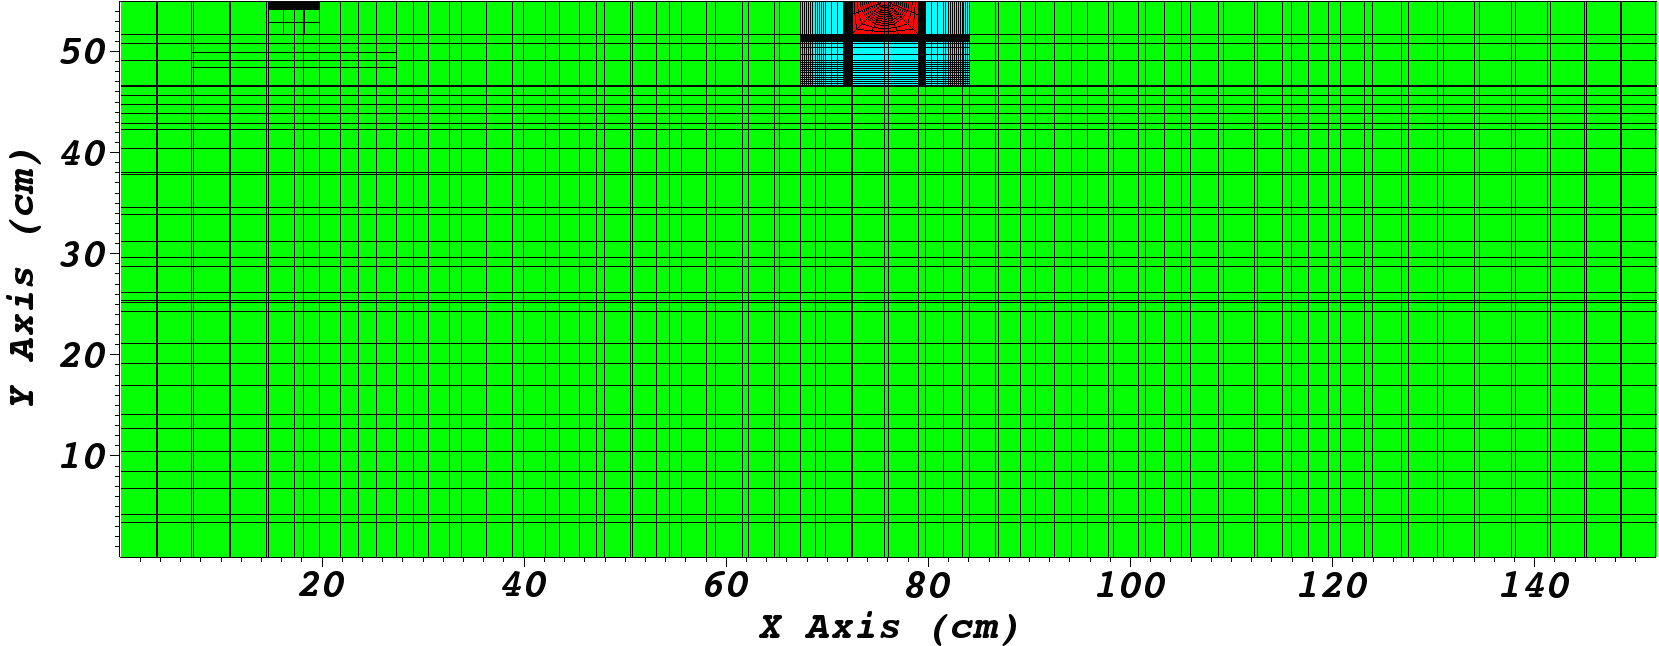
\includegraphics[scale=0.28]{../../figures/level2_42x13.png}
\caption{The Level-2 experiment mesh evenly partitioned into 42 subsets in x and 13 subsets in y. $f = 32.616$.}
\label{level2_42x13}
\end{figure}
\begin{figure}[H]
\centering
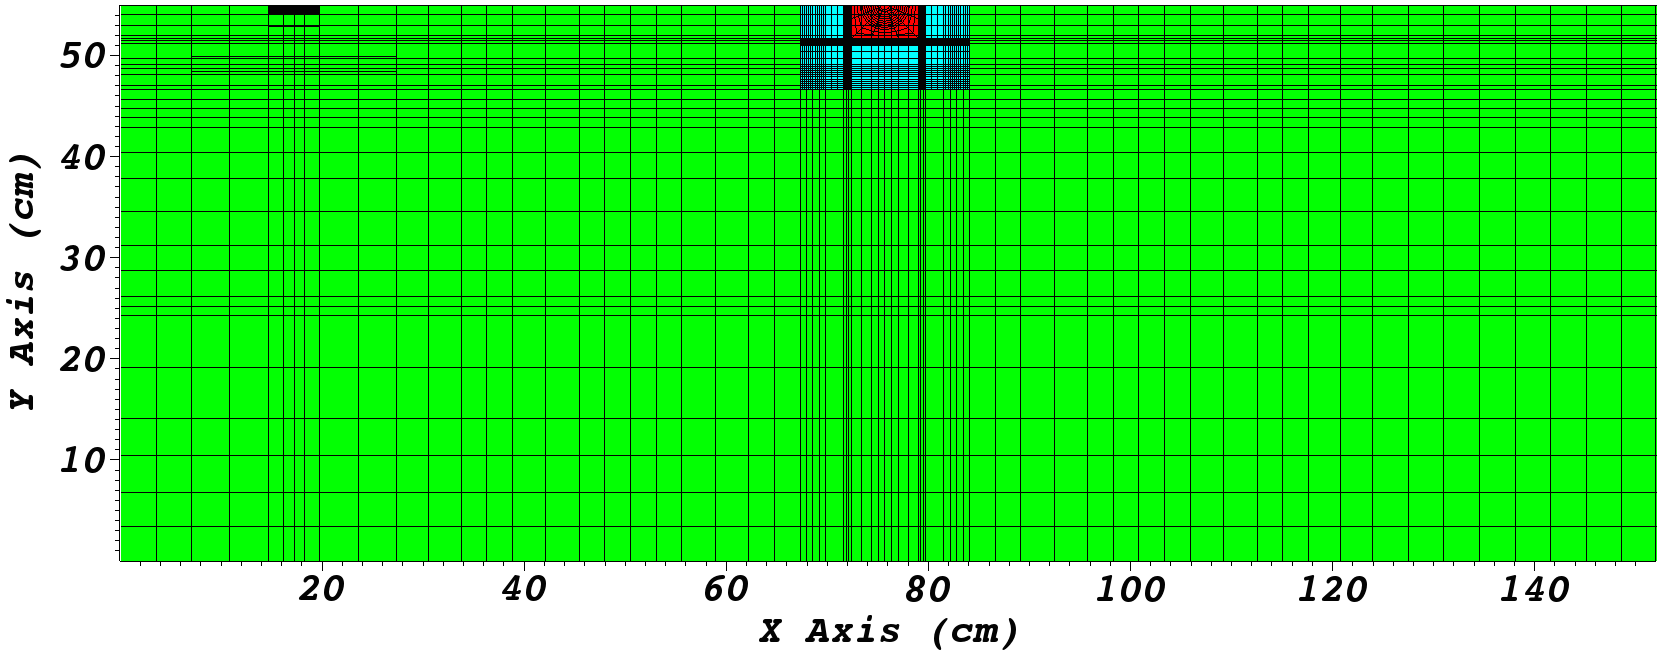
\includegraphics[scale=0.28]{../../figures/level2_42x13_balanced.png}
\caption{The Level-2 experiment mesh partitioned and manually load balanced with 42 subsets in x and 13 subsets in y. $f = 2.386$.}
\label{level2_42x13_balanced}
\end{figure}

Table \ref{level2_sweep_times} shows the sweep times for the regular cut and balanced cut Level-2 problems for PDT and the time-to-solution estimator. The minimum and maximum solve time per sweep values are also tabulated.
Table \ref{level2_percent_diff} shows the percent difference between the PDT sweep time and the time-to-solution estimator sweep time.
\begin{table}[ht]
\centering
\caption{The sweep times for the regular cut and manually balanced cut Level-2 problems for PDT and the time-to-solution estimator.}
\label{level2_sweep_times}
\begin{tabular}{c|c|c|c|c}
\bf Case & \bf PDT (s) & \bf TTS (s) & \bf PDT Min (s) & \bf PDT Max (s) \\ \hline
Regular & 0.07 & 0.0648 & 0.0686 & 0.0889\\ \hline
Manually Balanced & 0.0531 & 0.0535 & 0.0522 & 0.0638
\end{tabular}
\end{table}
\begin{table}[ht]
\centering
\caption{The percent difference for the regular cut and manually balanced cut Level-2 problems between PDT and the time-to-solution estimator.}
\label{level2_percent_diff}
\begin{tabular}{c|c}
\textbf{Case} & \bf PDT vs. TTS \\ \hline
Regular & 7.52\% \\ \hline
Manually Balanced & 0.63\%
\end{tabular}
\end{table}
Both the regular and balanced cases have estimated sweep times within 8\% of PDT's sweep times.
Because both of these problems have between 3,000 and 4,000 cells, the number of unknowns in the problem can mitigate the effects seen in the unbalanced pin cases.
The difference in schedule in addition to latency instabilities at 546 cores are less significant with larger problems.

In the future, the schedule from the time-to-solution estimator should be fed into PDT and see if the agreement improves.
In addition, the latency on a machine like Quartz is easy to mischaracterize.
A supercomputer of that size and in constant use can have differing latencies depending on how many nodes are in use and which particular nodes are in use.
The data generated for the scaling suite was done during dedicated access time, when latencies are much easier to characterize with only one user using the entire machine, explaining the good agreement out to 16,000 cores.

Additionally, the machine parameters were generated empirically using a serial suite of structured mesh problems.
In the future, obtaining machine parameters should be attempted using unstructured meshes, and agreement between PDT and the time-to-solution estimator restudied.

%\begin{figure}[ht]
%\centering
%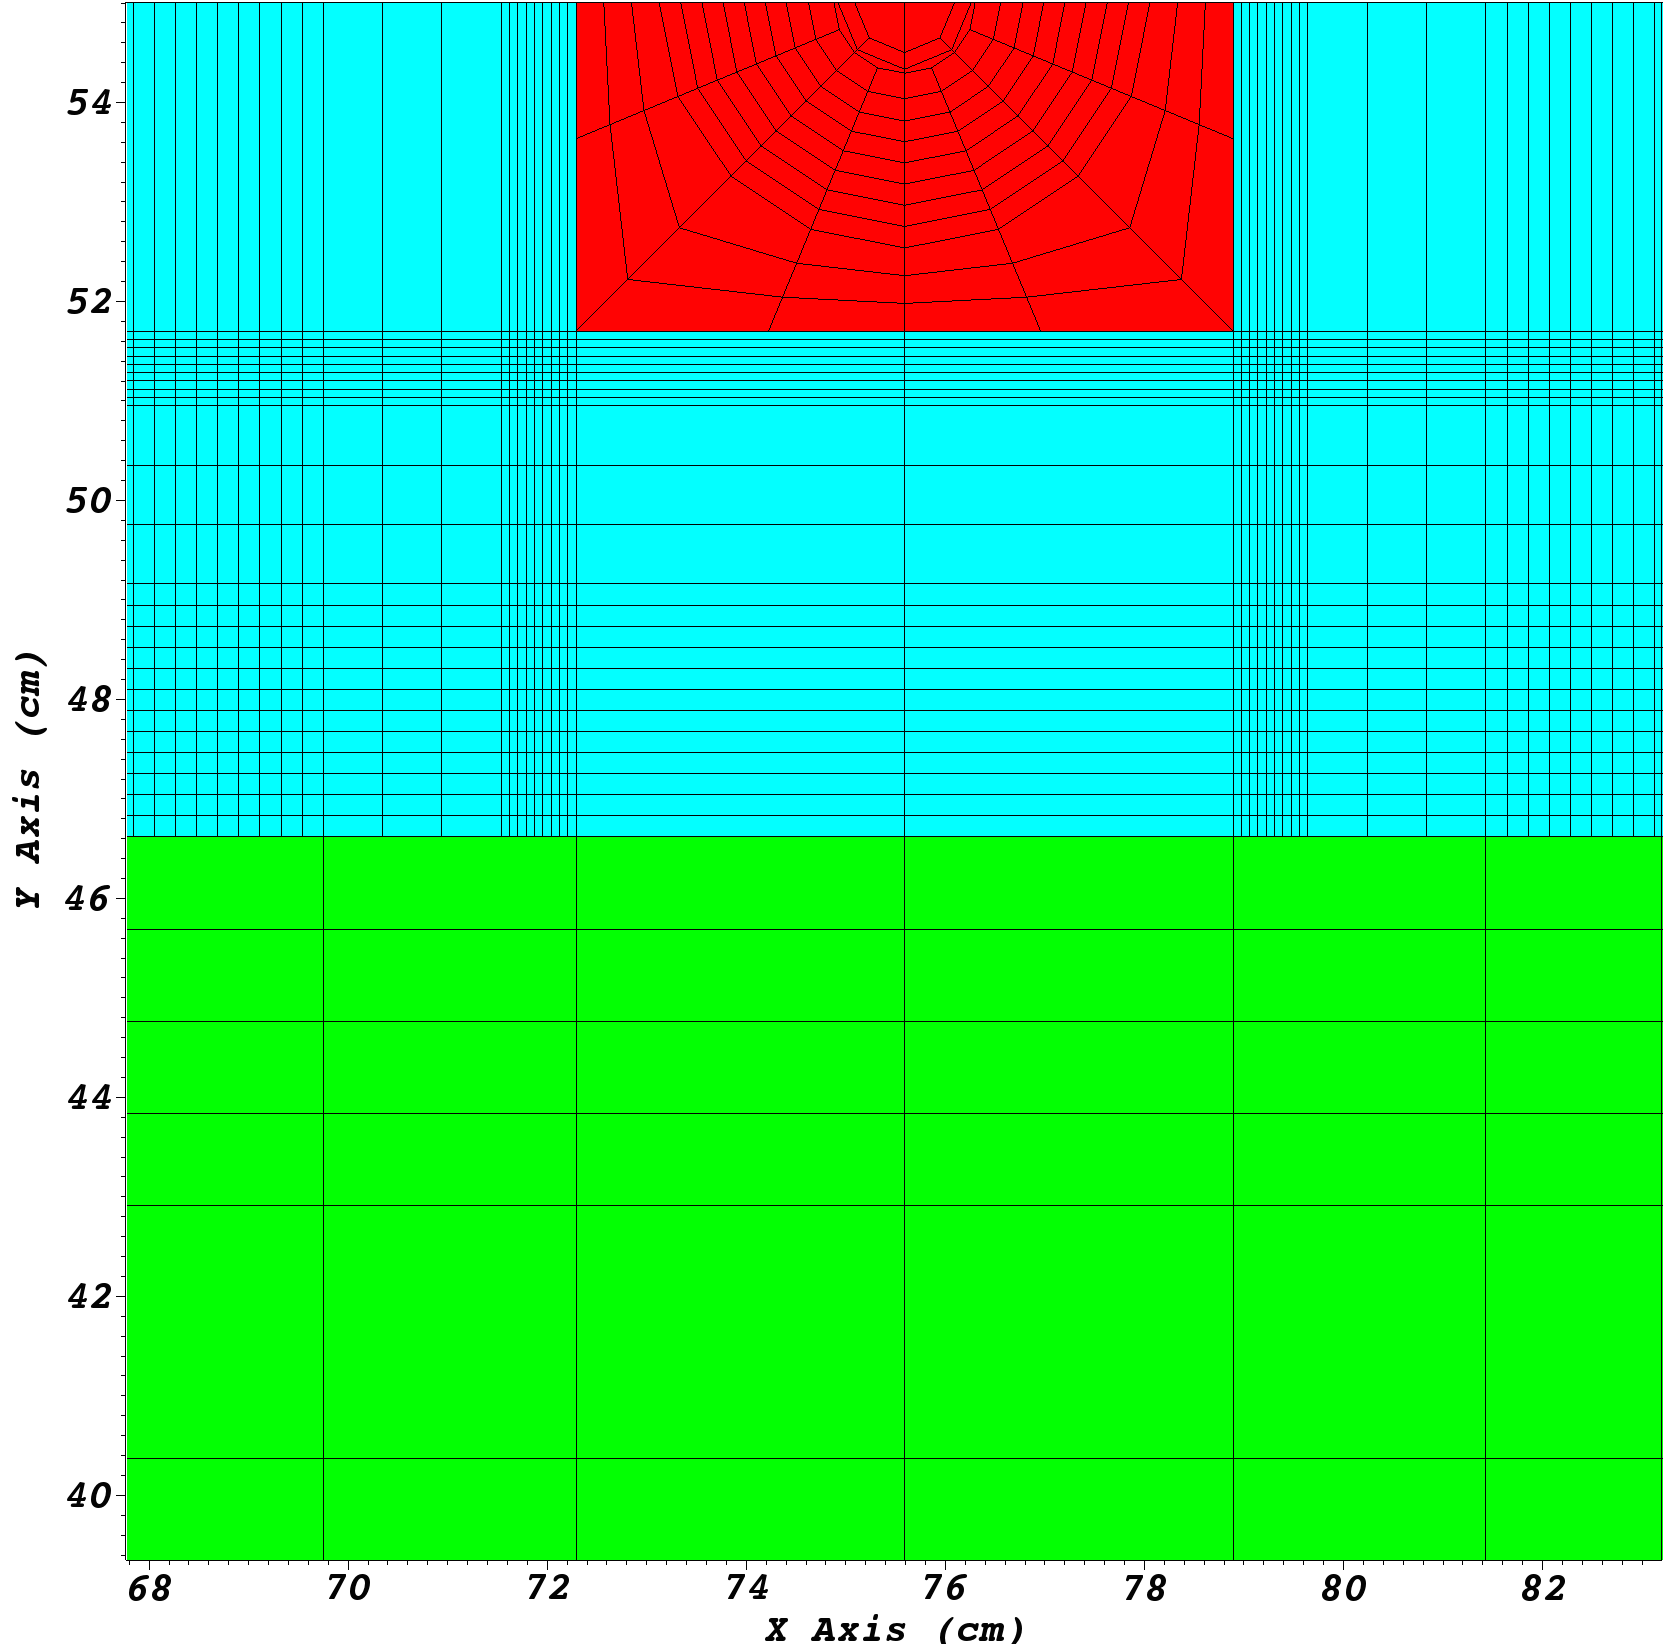
\includegraphics[scale=0.15]{../../figures/level2_nocut_zoom.png}
%\caption{The detector region of the Level 2 experiment mesh.}
%\label{level2_nocut_zoom}
%\end{figure}
%
%\begin{figure}[ht]
%\centering
%\includegraphics[scale=0.15]{../../figures/level2_42x13_zoom.png}
%\caption{The detector region of the Level 2 experiment when partitioned into 42 subsets in x and 13 subsets in y.}
%\label{level2_42x13_zoom}
%\end{figure}
%
%\begin{figure}[ht]
%\centering
%\includegraphics[scale=0.15]{../../figures/level2_42x13_balanced_zoom.png}
%\caption{The detector region of the Level 2 experiment when partitioned and balanced with 42 subsets in x and 13 subsets in y.}
%\label{level2_42x13_balanced_zoom}
%\end{figure}
